\chapter{ROBUST CLUSTERING of AD HOC COGNITIVE RADIO NETWORK}
\section{Introduction}
\label{intro}
%\todo[inline]{The first paragraph will be moved/integrated to INTRODUCTION chapter later.}
%\gls{CR} is a promising technology to solve the spectrum scarcity problem~\cite{Mitola}. 
%In CR systems, primary users access their allocated spectrum band whenever there is information to be transmitted. 
%In contrast, CR users (forming cognitive radio networks, abbreviated as CRN) can only access primary channels after validating the channel is idle. 
%This refers to the process of sensing a particular channel and verifying (with a previously specified probability of error) that it is not used by a primary user currently. 
%This form of spectrum sharing is also referred to as opportunistic spectrum access.

%[Benefits of clustering]





%[clustering in crn] 
As introduced in Chapter~\ref{INTRODUCTION}, efficient spectrum sensing is identified as to be critical to the success of cognitive radio networks~\cite{Sahai_FundamentalDesignTradeoffs2006}.
Cooperative spectrum sensing is able to effectively cope with noise uncertainty and channel fading, thus remarkably improves the sensing accuracy.~\cite{coorperativeSensing_Akyildiz11}.
Collaborative sensing relies on the consensus of CR users within certain area, and decreases considerably the false sensing reports caused by fading and shadowing of reporting channel.
Clustering, \ie forming adjacent secondary users as a collectivity to perform certain tasks together, is regarded as an effective method used in cooperative spectrum sensing~\cite{Sun07_clustering_spectrum_secsing, Zhao07}.
%As a result, more accurate sensing result can be obtained by collaborative sensing, and the improvement on spectrum sensing decreases the interference originating from CR users to primary users, which is highly desirable.
%Also,  prevents CR users from using channels that are occupied by primary users. 
Clustering is also efficient to enable all CR users\footnote{User and node are used interchangeably in this chapter} within the same cluster to stop payload transmission on the operating channel and initiate the sensing process, so that the all the CR nodes within the one cluster are able to vacate the channel swiftly when primary users are detected by at least one CR node residing in the cluster~\cite{willkomm08}.
With cluster structure, as CR users can be notified by cluster head (\gls{CH}) or other cluster members about the possible collision, the possibility for them to interfere neighbouring clusters is reduced~\cite{centralizedSharing80222}. 
Clustering algorithm has also proposed to support routing in cognitive ad-hoc networks~\cite{Abbasi_survey_07}.

%%[crn for clustering] 
%%due to attenuation of signal propagation, primary users can only be detected by CR users when they locate closely to CR users.
%In cognitive radio networks, secondary users which locate closely with each other are possibly affected by the same group of primary users, so that the availability of licensed spectrum is similar to them, \ie certain channels are available on each of them.
%The similarity of available spectrum on a group of neighbouring CR nodes, along with the benefit of collaborative decision among multiple nodes, leads to clustering as an effective approach for many applications.

%[robustness issue for clustering]
Except for the advantages brought in by clustering, there is an issue on forming clusters in cognitive radio network.
As the activity of primary users is controlled by licensed operators which are generally not known to CR nodes, the communication on licensed channels between CR nodes is not guaranteed. 
For a pair of communicating CR nodes, whenever a primary user is detected to be operating on the working channel, CR nodes have to retreat that working channel.
The affected CR nodes switch to one other idle channel if there are available idle channels, if not, the communication has to be stopped.
As a result, when coexisting with primary users, the ability for one pair of CR nodes to maintain communication on licensed channels is totally decided by primary users' activity.

Although the formed clusters is vulnerable under the influence of primary users, and there is little possibility to change primary users' operation, there is something can be done by secondary users in the process of forming clusters. 
One cluster is sustained when there is at least one common channel available for all members in that cluster, so that the cluster can operate on the licensed channel.
As the increase of channel occupation by primary users is assumed to be random, a cluster with more channels will survive with higher probability.
Thus the number of available common channels in the cluster indicates robustness of it when facing ungovernable influence from primary users.
It is not difficult to see that forming clusters with different neighbours leads to different amount of common channels in the clusters.
As a result, how to form the clusters plays an important role on the robustness of clusters in CRN.

%Furthermore, the clustering algorithm also determines the connectivity between several clusters which ultimately determines the robustness of the entire network on the respect of connectivity. 

To solely pursue cluster robustness against the primary users' activity, \ie to achieve more common channels within clusters, the ultimately best clustering strategy is ironically that each node constitutes one single node clusters.
%In that case, the common channels within cluster are the available channels available at that node's place.
Apparently this contradicts our motivation of proposing cluster in cognitive radio network.
This contradiction indicates that, the robustness discussed in terms of number of common channels carries little meaning when the sizes of formed clusters are not given consideration.
Besides, cluster size plays import roles in certain aspects.
For instance, cluster size is one decisive factor in power preservation~\cite{clustering_globecom11, EnergyEfficientClusteringRouting_2015}, and it is also influence the accuracy of cooperative spectrum sensing~\cite{Consensus_based_clustering12}.
Hence, cluster size should be given consideration when discussing cluster robustness against primary users.

In this chapter, a decentralized clustering approach ROSS is proposed to cover the issue of robustness of clusters in CRN.
ROSS is able to form clusters with desired sizes, and the generated clusters are more robust than other robust clustering schemes, \ie more secondary users residing in clusters against increasing influence from primary users.
Compared to previous work, ROSS involves much less control messages, and the generated clusters are significantly more robust.
ROSS selects cluster head through coordination within its neighborhood, and then cluster membership is decided locally and its fast convergence is proved under game theoretic framework. 
%building more homogeneous clusters with respect to their size and forcing nodes with a high connectivity degree to the border of a cluster (making the cluster therefore more robust regarding connectivity loss to its neighbor).
%For our scheme we can prove convergence in cluster formation phase and resolve ambiguities with respect to cluster membership in a game-theoretic setting. 
On the basis of ROSS, we propose a light weighted version \gls{ROSS-DFA} which requires exchanging less overheads.
Throughout this chapter, we refer both \gls{ROSS-DGA}, ROSS-DFA, and the other versions with size control feature, as \textit{variants of ROSS}. 

The rest of chapter is organized as follows. 
After reviewing related work in section~\ref{related_work}, we present our system model in Section~\ref{sec:model}. 
Then we introduce our clustering scheme ROSS and its variants in section~\ref{ross}.
Centralized scheme is given discussion in section~\ref{centralized_scheme}.
Performance evaluation is in section~\ref{performance}.
Finally, we conclude our work and point out direction future research in section~\ref{conclusion}.


\section{Related Work}
\label{related_work}

Prior to the emergence of open spectrum access, as an important method to manage network, clustering has been proposed in for ad hoc networks~\cite{Kawadia03,Lin97adaptiveclustering,Basagni99}, wireless mesh networks~\cite{Abbasi_survey_07}, and wireless sensor networks~\cite{Abbasi_survey_07} and . 
In ad hoc and mesh networks, the major focus of clustering is to preserve connectivity (under static channel conditions) or to improve routing.
In the context of sensor networks, the emphasis of clustering has been on longevity and coverage.
Overhead generated by clustering in ad hoc network is analysed in~\cite{clusterRoutingOverhead02infocom, clusterRoutingOverhead_wcnc04}.



As to cognitive radio networks, clustering schemes are also proposed, which target different aspects.
Work~\cite{Consensus_based_clustering12} improves spectrum sensing ability by grouping the CR users
with potentially best detection performance into the same cluster.
Clustering scheme~\cite{clustering_globecom11} obtains the best cluster size which minimizes power consumption caused by communication within and among clusters.
\cite{clustering_globecom11} proposes clustering strategy in cognitive radio network, which looks into the relationship between cluster size and power consumption and accordingly controlling the cluster size to decrease power consumption.
%The works~\cite{} introduced in Introduction section don't provide solution that how are the clusters formed.
%There have been several clustering schemes tailored for CRNs. 
Cogmesh is proposed in~\cite{Chen07} to construct clusters by the neighbour nodes which share local common channels, and by interacting with neighbour clusters, a mesh network in the context of open spectrum sharing is formed.
Robustness issue is not considered by this clustering approach.
\cite{TWC2012_cooperative_communication} targets on the QoS poisoning and energy efficiency. 
This approach first decides on the relay nodes which minimize transmission power consumption, then the chosen nodes become cluster heads and clusters are formed in a dynamic coalition process.
This work emphasis on power efficiency and doesn't take into account the channel availability and the issue of robustness of the formed clusters.
In~\cite{Zhao07, Affinity_clustering_09icccn}, the channel available to the largest set of one-hop neighbours is selected as common channel which yields a partition of the CRN into clusters. 
This approach minimizes the set of distinct frequency bands (and hence, the set of clusters) used as common channels within the CRN.
However, bigger cluster sizes generally lead to less options within one cluster to switch to if the common channel is reclaimed by a primary node. 
Hence, this scheme does not provide robustness to formed clusters. 
\cite{cluster_EW10} deploys cluster structure in order to implement common channel control, medium access  with multiple channel and channel allocation. 
The node with the maximum number of common channels within its k-hop neighborhood is chosen as cluster head, but how to avoid one node appearing in multiple clusters is not given consideration.

Clustering robustness is considered in ~\cite{Lazos09, LIU_TMC11_2}.
Authors~\cite{Lazos09, LIU_TMC11_2} emphasis on improving the numbers of common channels within clusters,   in order to strengthening robustness of clusters, but the perused metric is not examined or proved to be able to sustain cluster structure.
The authors consider the balance between the number of idle common channels within cluster and cluster size and propose an algorithm that increases the number of common channels within clusters. 
%However, this work neglects the issue of connectivity between clusters. 
One drawback of this scheme is, in order to increase the number of common channels within clusters, the scheme excludes certain CR nodes from the formed clusters, so that isolated nodes have to form clusters themselves. 
Besides, this scheme leads to a high variance on the size of clusters, which is not desired in certain applications as discussed in~\cite{clustering_globecom11, cluster_EW10}.



\section{System Model}
\label{sec:model}
Let us consider a two dimensional area where primary and secondary users coexist together.
\subsection*{Spectrum sensing and etiquette}

The set of primary users and secondary users are presented by $\mathcal{P}$ and $\mathcal{N}$ separately, and there are $|\mathcal{P}| = P$ and $|\mathcal{N}| = N$.
The collection of non-overlapping licensed frequency bands is denoted as $\mathcal{F}$ with $|\mathcal{F}| =F$.
We assume that primary users have a relatively low variation in activity (periods of activity and inactivity in the range of seconds or minutes).
CR users have the same transmission range on both licensed and control channel.
Primary users also have fixed transmission range on the licensed channels\footnote{This assumption is made to simplify the discussion, and doesn't affect the effectiveness of the proposed scheme}.
As to two secondary users, if the distance in between them is smaller than secondary users' transmission range, we assume the pair is able to communicate on both control channel and licensed channel, and the both are considered to be neighbours of each other.
%If one secondary user locate within a certain primary user's transmission, we regard this secondary user to be able to 

Primary users access the allocated channels in $\mathcal{F}$ according to its need without sending any explicit notification to secondary users.
Secondary users conduct spectrum sensing independently, by which the secondary users validate the channels to be available or not. \footnote{The spectrum availability can be validated with a certain probability of detection. Spectrum sensing/validation is out of the scope of this thesis.}
%as well as with a certain periodicity, i.e., every $T_{\mathrm{sense}}$ time the currently used channels need to be validated again.
The available channels sensed on secondary user $i$ is denoted by $V_i$ and $\vert V_i \vert \leq F$. % indicating the total number of available channels for CR user $i$.
%Each secondary user notifies its neighbours of the sensing result about the available channels.


Any user outside the transmission range of the transmitter can not receive data from it, \ie  any CR user outside primary users' transmission ranges can not detect their existence, whereas a CR user can always communicate with CR sender, or detect the operating primary user, when it locates within the CR sender or the operating primary user's transmission range.
As the transmission range of primary users is limited and secondary users are at different locations, secondary users have different views on the occupancy of the spectrum (apart from the fact that there might be false negatives in the sensing process), i.e., $V_i \neq V_j$, for $i \neq j$.
One dedicated control channel is assumed to be available for all the CR nodes to exchange control messages with neighbours in the process of cluster formation.
The control channel could be in ISM band or other reserved spectrum which is exclusively used for transmitting control messages.
Note that the assumption of dedicated control channel is to simplify the discussion so that we can focus on the kernel of this chapter, robustness of clusters.
%One control channel makes a CR user to establish a link for communication with its neighbours.
Actually, the control messages involved in the clustering process can be conveyed on available licensed channels through rendezvous process by channel hopping~\cite{channelHopping_Rendezvous_2014, Gu_distributed_rendezvous_2014}. 
The transmission range of CR user on control channel is identical with that on licensed channel.
Over the control channel, secondary users exchange their spectrum sensing results $V_{i}$ with one hop neighbours. 

\subsection*{Cognitive radio network}
Cognitive radio network is constituted by all the secondary users in $\mathcal{N}$.
%Neighbourhood establishment and maintenance with control channel and according to a neighborhood discovery protocol which is out of scope of our work.
When licensed channels are available on two neighbouring secondary nodes in the same time, payload communication can be conducted on one or multiple licensed channels.
%While primary users are assumed to be fixed, secondary users can be mobile.
%Validation refers to the process of ensuring that no primary transmission is actually taking place on the respective channel.
%All $N$ secondary users constitute an ad-hoc network in which data can be transmitted from one certain node to any other node should available c.hannels are available on the source node, destination node and other intermediate nodes.
%Communication on licensed channels is possible only when nodes $i, j$ are both located in each other's transmission range and both share a validated licensed channel.
Due to the assumed $0/1$ state of connectivity solely based on distance between CR users, the CRNcan be represented by a connectivity graph $\mathcal{G}(I,\mathcal{E})$, where $\mathcal{E}=\lbrace(i,j,v) \vert i, j \in \mathcal{N} \wedge v\in V_i \wedge v\in V_j \rbrace$ is wireless link between any secondary node $i$ and its neighbour $j$ with licensed channel $v$.
Due to relatively low primary user dynamics, time index is omitted here.


%In order to perform clustering, CR users first need to establish their neighborhood.
For secondary node $i$ in CRN, its neighborhood $Nb_i$ consists of all the secondary users locating within its transmission range (links are assumed to be reciprocal), regardless whether common licensed channels exist or not. 
% and have at least one common channel with node $i$ each, i.e. $ j\in Nb_i \Rightarrow V_i\cap V_j\neq \emptyset$.
%The clustering phase is initialized during which any control message is again conveyed by the control channel.
In the rest of this chapter, \textit{channel} only refers to the licensed spectrum except when control channel is particularly mentioned.

\subsection*{Clustering}
A cluster $C$ is composed with one cluster head and cluster members, which satisfies the following conditions:

\begin{itemize}
\item Cluster head $H_C$ is able to communicate with any cluster member directly, \ie for any cluster member $i\in C$, there is $i\in Nb_{H_C}$.
\item There exists as least one common licensed channel for the cluster, \ie $\cap_{i\in C} V_i \neq \emptyset$.
\end{itemize}
%A cluster has four items: A cluster head, cluster members, common channels of the members with the head and the one channel currently used for payload data transmission.
Cluster head coordinates the activities of cluster members, \ie notifies all the members to evade a channel if the channel is sensed by one cluster member to be occupied by primary users, or notify the members to use a different channel for payload communication. 
Cluster is denoted as $C_i$ when its cluster head is $i$.
%, for the sake of concision, $C_i$ is also named as cluster $i$ in the following part of this chapter.
We refer to the common channels within a cluster $C$ by the term \textit{common control channels} (\gls{CCC}) and denote this set of channels by set $K_C$.
$ K_C = \cap_{i\in C_i} V_i$, and $k_C = |K_C|$ is the number of common channels for cluster $C$.
As the CR users are potentially mobile, clustering is performed with some periodicity, but obviously not more often than spectrum sensing.



%We propose distributed scheme ROSS to form clusters to generate robust clusters, and in the same time clusters have preferred sizes, \ie fewer number of singleton clusters (the cluster which consist with only one CR node) compared with state of art.

%Besides, cluster size is also considered in to clustering solution.
%Size preference can be met after minor modifications on ROSS.


%The metric is summation of the number of channels available to be used for each node when they reside in a certain cluster, together with a cost for not following the desired cluster size, \ie when the desired cluster size is $\delta$ and the other cluster sizes are denoted as $\delta'$, the metric is, 
%\begin{equation*}
%\label{metric}
%\sum_{i=1}^{N}(ICC_i)
%\end{equation*}
%$N$ is the number of CR nodes in the network.


%Also, we refer to the common channels between neighbouring clusters by the term \textit{outward common channels} (OCC). We define the set of OCCs of cluster $C$ to be the set of available common channels between any member of $C$ and any other CR user of a neighbouring cluster:
%\begin{equation*}
%\label{numocc}
%R_{C}=\bigcup_{j\in C, k\in N_j, k\notin C}(V_{j}\cap V_{k})
%\end{equation*}

%In the process of clustering, when there is no restriction on cluster size, the metric will only be the summation of the number of channels for each node when they reside in a certain cluster.
%When we try to maximize the summation of ICCs, an obvious correlation between cluster size and number of ICCs is encountered, \ie when each node constitutes one cluster, the aforementioned metric will be maximized.
%The goal of the proposed clustering scheme is to let as more CR nodes as possible to form clusters, meanwhile the clusters have more common channels and preferred cluster size.

\begin{table}[ht!]
\caption{Notations in robust clutering problem}\label{tab1}
\centering
\begin{tabular}{llr}
\toprule
%\multicolumn{2}{c}{Item} \\
%\cmidrule(r){1-2}
Symbol & Description \\
\midrule
$\mathcal{P}$, $\mathcal{N}$  & complete collection of primary and secondary users\\
%$J$ & set of primary uesrs in the scenario\\
$\mathcal{F}$ & set of non-overlapping channels in the scenario\\
$Nb_i$ & node $i$' neighborhood     \\
$C$ & a cluster \\
$V_i$   & set of available channels on CR node $i$  \\
$V_C$   & set of available common channels of cluster $C$  \\
$V_{C_i}$   & set of available common channels of cluster $C$ whose cluster head is $i$\\
%$\phi_i$ & the number of available channels for cluster $i$\\ 
%		& note it is different than $|V_i|$\\
%$p_i$   & number of available channels on CR node $i$  \\
$C_i$ & a cluster whose cluster head is $i$ \\
& there is an exception: in Section~\ref{centralized_scheme}, $C_i$ is $i$th cluster among the legitimate clusters.\\
$H_C$ & cluster head of a cluster $C$\\
$\delta$ & desired cluster size\\
%$C_i$ & a cluster with CR node $i$ as cluster head \\
%$V_{C_i}$   & set of common channels within cluster $C_i$  \\
%$V_{OC_i}$   & set of common channels among cluster $C_i$ and neighbor clusters  \\
%$CH_i$ & cluster head of node $i$ \\
%$CHS_i$ & set of cluster heads of node $i$ after phase I\\
$S_i$ & set of claiming clusters, each of which includes \\
& debatable node $i$ after phase I\\
$K_{C_i}$ & set of common channels within cluster $C_i$\\
$k_{C_i}$ & number of common channels of cluster $C_i$\\
%$m_{ij}$ & number of common channels between CR node \\
%& $i$ and $j$\\
\bottomrule
\end{tabular}
\end{table}





\section{Distributed Coordination Framework: Clustering Algorithm}
\label{ross}
%Despite this fact, as some features brought by clustering structure are valued as said in introduction section, the clustering scheme which groups certain CR nodes together and meanwhile produces robust connectivity will be proposed.

%Thus, the number of common channels should be the only metric for clustering schemes.


In this section, we present the new clustering scheme named \gls{ROSS} (RObust Spectrum Sharing). It is based on the local sensing results $V_{i}$ of all CR users $i$ and utilizes local similarity of the available channels to form clusters. ROSS consists of two cascaded phases: \textit{cluster formation} and \textit{membership clarification}. We will describe both phases sequentially.

\subsection{Phase I - Cluster Formation}
After spectrum sensing and communication with neighbours, every CR node is aware of the channel availabilities on itself and all its neighbours.
We propose two metrics for each CR node to characterize the channel availability between it and its neighborhood.
%\newtheorem{def1}{Definition}
%\label{def1}
%\begin{def1}
%Connection vector $\left\{D_i,G_i\right\}$ of CR node $i$:
%spectrum connectivity degree: 
%\begin{equation}
%\label{D_i}
%D_i=\sum_{j\in N_i}\vert V_i\cap V_j\vert
%\end{equation}
%Social Connection degree:
%\begin{equation}
%\label{G_i}
%G_i=|\bigcap_{j\in N_i}V_j|
%\end{equation}
%\end{def1}

\textit{Individual connection degree} $D_i$: $D_i=\sum_{j\in Nb_i}\vert V_i\cap V_j\vert$, which denotes the sum of the pairwise common channels of node $i$, and is an indicator of node $i$'s adhesive property to the CRN. 

\textit{Social connection degree} $G_i$: $G_i=|\bigcap_{j\in Nb_i}V_j|$, which is the number of common channels in $Nb_i$. $G_i$ represents the ability of $i$'s neighborhood to form a robust cluster. Figure~\ref{fig1} illustrates an example CRN where the corresponding individual and social connection degrees are specified for each node.
\begin{figure}[ht!]
  \centering
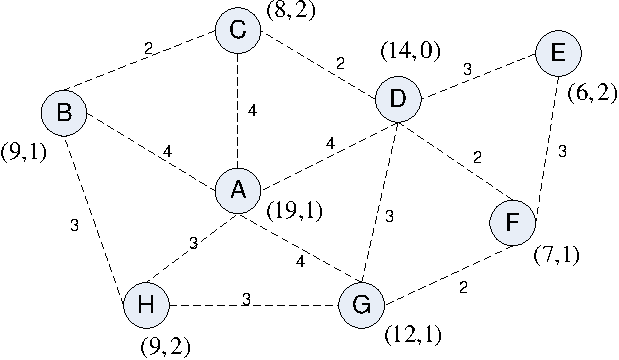
\includegraphics[width=0.6\linewidth]{figure1.pdf}
% 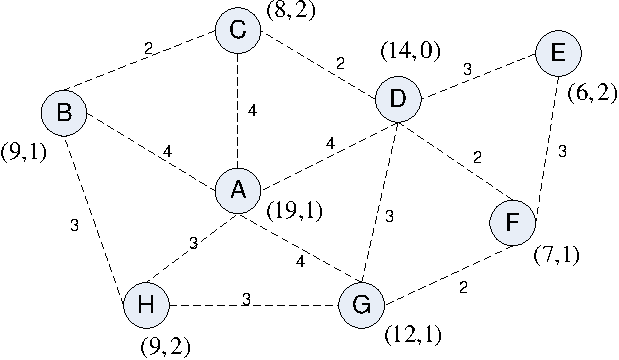
\includegraphics{figure1.pdf}
	\caption{Connectivity graph and the connectivity vector $\{D_i, G_i\}$ on each node. The available channels sensed by each CR node are: $V_A=\{1,2,3,4,5,6,10\}, V_B=\{1,2,3,5,7\}, V_C=\{1,3,4,10\}, V_D=\{1,2,3,5\}, V_E=\{2,3,5,7\}, V_F=\{2,4,5,6,7\}, V_G=\{1,2,3,4,8\}, V_H=\{1,2,5,8\}$. Dashed lines indicates two end nodes are within transmission range of each other. Each edge is labelled by the number of common channels between the two ends.}
	\label{fig1}
\end{figure}

The algorithm of phase I can be sketched like this: cluster heads are determined firstly, accordingly clusters are formed with cluster head's neighbourhood.

\subsubsection*{Determining Cluster Heads}
In this phase, each CR node decides whether it is cluster head by comparing relevant metrics with its neighbours.
Briefly speaking, the CR node which has the biggest \textit{individual connection degree} in its neighbourhood excluding already decided cluster heads becomes cluster, \ie CR node $i$ becomes cluster head if $D_i<D_k, \forall k\in Nb_i\setminus CHs$ ($CHs$ donate the cluster heads existing in $Nb_i$).
If there is another CR node $j$ in its neighborhood has the same \textit{individual connection degree}, \ie $D_j = D_i$, furthermore $D_j < D_{k}, \forall k\in Nb_j\setminus \{CHs\cup i\}$, then the node out of $\{i, j\}$ with higher \textit{social connective degree} becomes cluster head, and the other one becomes member of it. 
If $G_i = G_j$ as well, node ID is used to break the tie, \ie the one with smaller node ID takes precedence and becomes cluster head.
%This algorithm is contradictory to intuition by choosing the node with smallest $D_i$ as cluster head.
%The reason is that, by deciding cluster head in this way, the CR node with bigger $D_i$ will locate at the edge of clusters, and as they have higher \textit{Individual Connection Degree}, they are more likely to be integrated into one certain cluster, thus less singleton clusters are formed.

The pseudo code of phase I of clustering is in Algorithm~\ref{alg0}.
\begin{algorithm}              % enter the algorithm environment
\caption{Cluster head determination and cluster formation}          % give the algorithm a caption
\label{alg0} 
\DontPrintSemicolon
\SetAlgoLined
\KwIn{Unclustered CR node $i$ which is aware of $D_j$ and $G_j$, $j\in Nb_i$, and the ID of CRs which have be decided to be cluster heads, $ID_{CH}$, $CH\in Nb_i$. Empty sets $\tau_1,\tau_2,\tau_3,\tau_4,\tau_5$}
\KwResult{Whether or not $i$ is cluster head}
\For{CR node $j\in Nb_i\setminus CHs$}{
\eIf{$D_i==D_j$}{
	$\tau_1\leftarrow j$
	}
	{\If{$D_j < D_i$}{
		$\tau_2\leftarrow j$
		}
	}
	}
\uIf{$\tau_2 \neq \emptyset$}{
	$i$ is not CH; break;
	}
\uElseIf{$\tau_1$ is $\emptyset$}{
	$i$ is CH; break;
	}
\Else{ 	
\tcc*[r]{$\tau_1 \neq \emptyset, \tau_1 == \emptyset$}\mbox{}
	\For{$\forall k \in \tau_1$}{
	\If{$\nexists m\in Nb_k\setminus CHs$, such that $D_m < D_k$ }{
		$\tau_3 \leftarrow k$
		}
	}
	\eIf{$\tau_3$ is $\emptyset$}{
		$i$ is CH;break;
		}{
		\For{$\forall n\in \tau_3$}{
			\eIf{$G_n > G_I$}{
				$\tau_4 \leftarrow n$}{
				\If{$G_n == G_i$}{
				$\tau_5 \leftarrow n$
				}
			}
			}
		\uIf{$\tau_4 \neq \emptyset$}{
			$i$ is not CH;break;
			}
		\uElseIf{$\tau_4$ is $\emptyset$ and $\tau_5 \neq \emptyset$}{
		\If{$ID_i < ID_r, \forall r\in \tau_5$}{$i$ is CH;break;}	
		}
		\Else{$i$ is CH;break;\tcc*[r]{$\tau_4$ and $\tau_5$ are $\emptyset$}}
	}
}
\If{$i$ is cluster head}{
	$D_j, j\in Nb_i\setminus CHs$ is changed as a big positive value $M$;
	}
\end{algorithm}


\subsubsection*{Initial Cluster Formation}
After deciding itself being cluster head, CR node broadcasts to notify its neighbours on control channel, meanwhile, $i$'s initial cluster is formed immediately, which is $i$'s neighborhood except for those nodes which have become cluster heads, \ie $C_i=(Nb_i\setminus CHs)\cup i$.
It is possible that the formed cluster doesn't poses inner common channel, this can be handled in the following way. 
As smaller cluster size increases the number of common channels within the cluster, certain nodes are eliminated until there is at least one common channel.
The elimination of nodes is performed according to an ascending list of nodes sorted by their number of common channels with the cluster head, which means, the cluster member which has the least common channels with the cluster head will be excluded first.
If there are nodes having the same number of common channels with cluster head, the node whose elimination brings in more common channels will be excluded.
If this criterion meets a tie, the tie will be broken by deleting the node with smaller ID.
It is possible that the cluster head excludes all its neighbours and resulting itself to be the cluster.
%At the end of this procedure every formed cluster has at least one common channel.
Figure~\ref{fig1} depicts an example how CR nodes decide cluster heads. 
Node $B$ and $H$ have same individual connection degree, $D_B=D_H$, but as $G_H=2>G_B=1$, node $H$ becomes cluster head.
In Figure \ref{fig1}, the cluster $C_H$ is $\{H, B, A, G\}$.

As to the nodes eliminated in this procedure, they become either cluster heads or get included into other clusters later on, which is addressed in the following. 

After receiving the notification from a cluster head, a CR node is aware it is one member in a cluster, then the CR user changes its individual connection degree to be a big positive value $M$ (can be regarded as a positive infinite value), which is bigger than all the possible individual connectivity degrees in the CR network.
Then this CR user broadcasts this new individual connection degree to all its neighbours. 
If a CR node $i$ is associated to multiple clusters, $D_i$ is still set to $M$. %Note here that connectivity degree on cluster head will still be the actual value.% The value will expire after some duration and is changed later on back to the original value. 
When the cluster member is excluded from the cluster, its individual connection degree is restored to the original value which is further broadcast to its neighbours.
The purpose of manipulation on individual connection degree is to make the CR nodes out side this cluster possible to become cluster heads, so that every CR node either becomes cluster head or a member of at least one cluster.
The final states of all the CR users in the CRN are described in the following theorem.
%This judgement is conducted periodically, and phase I ends after every node ascertains it is cluster head or not.
\begin{lemma}
\label{clustering:lemma}
Every node in CRN will be included into at least one cluster in phase I in finite steps.
\end{lemma}

\begin{proof}
To see this, assume there are some nodes not assigned to any cluster and node $\alpha$ is one of them. As node $\alpha$ is not contained in any cluster, there must be at least one node $\beta\in Nb_\alpha$, with $D_{\beta} < D_{\alpha}$. Thus, node $\beta$ has at least one neighbouring node $\gamma$ with $D_{\gamma}<D_{\beta}$, and this series of nodes with monotonically decreasing $D_i$ might continue but finally ceases because the total number of nodes is limited. Now we find the last node $\omega$ in this series, because $\omega$ is the end node and does not have neighbouring nodes with smaller connectivity degree $D$, so $\omega$ will become a cluster head and embrace all its one-hop neighbours, including the node before it in the node series (here we assume that every new formed cluster has common channels). After that, the node recruited into cluster will set its connectivity degree $D$ to $M$, which enables the node further down in the list to become a cluster head. In this way, all the nodes in the series are included in at least one cluster in an inverse sequence. This clearly contradicts the initial assumption and proves the claim stated above. The proof implicitly shows that, within $\vert I \vert$ steps, all nodes will become a part of certain clusters and so phase I converges.
\end{proof}
According to Lemma~\ref{clustering:lemma}, we can assign reasonable amount of time for phase I to complete.
The pseudo code for cluster head to obtain at least one common channel is shown in Algorithm~\ref{alg_size_control_available_CCC}.



\subsubsection*{Cluster Size Control in Dense CRN}
\label{cluster_pruning}

In the introduction section, we have stated that cluster size should be given consideration to justify the pursuing of robust clusters, here we illustrate the pressing necessity to control cluster size when CRN becomes dense via theoretical analysis and simulation, and provide solution to it.

Assume CR nodes and primary users are evenly distributed and primary users occupy the licensed channels randomly, \ie both CR nodes density and channel availability in the CRN is homogeneous.
Based on Algorithm~\ref{alg0}, cluster heads are the CR nodes which poses the biggest individual connection degree in their neighborhood, and they are surrounded by CR nodes.
In contrast, CR nodes residing on edge are unlikely to become cluster heads as their neighbourhoods are only half the nodes locating away from edge.
The clusters formed are the neighborhood of cluster heads, which is decided by the transmission range and network density.
When this CRN becomes extremely dense, assume one cluster is formed by CR node $i$, based on the rule for cluster head selection Algorithm~\ref{alg0}, the nearest cluster head generated could locate just outside the neighborhood or transmission range of $i$, which is as Figure~\ref{clusters_denseNetwork} shows.
%
In the figure, black dots represent cluster heads, the circles denotes the transmission ranges of those cluster heads.
Cluster members are not shown in the figure.
%Circles represent the transmission range of cluster head, within which CR nodes are absorbed in cluster.
\begin{figure}[h!]
  \centering
  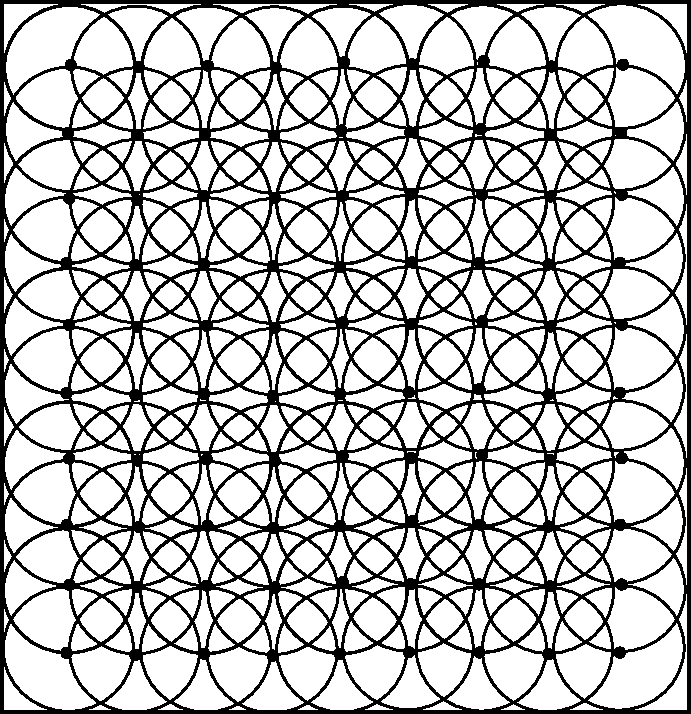
\includegraphics[width=0.5\linewidth]{clusters_denseNetwork_2.pdf}
  \caption{Clusters formation in extremely dense CRN. Black dots are cluster heads, cluster members are not drawn.}
  \label{clusters_denseNetwork}
\end{figure}
Let $l$ be the length of side of simulation plan square, and $r$ be CR's transmission radius.
Based on the aforementioned analysis and geometry illustration as Figure~\ref{clusters_denseNetwork}, we give an estimate on the maximum number of generated clusters as $l^2/r^2$.

Now we show the estimation is valid with simulation.
We distribute CR users and primary users randomly on a square plan, and set $r=10, l=50$.
Network density is increased by adding more CR users.
For each network scale, simulation is run for 50 times.
%We now have a look at how does the network density affect the cluster size when the transmission range is constant.
%This implicates when the cluster size is decided by the density of the network.
%As to SOC, the membership of one cluster is decided after a complex process, and the cluster size is roughly the same with one neighborhood.xxxx
%We can see from the example that although two neighbouring clusters can overlap greatly with each other, no cluster head will be covered by other clusters.
Figure~\ref{number_clusters_scale} shows the number of formed clusters.
With the increase of CR users in the network, network density increases linearly (see the right hand side Y axis, which indicates the number of neighbours.), and the number of formed clusters also increases and approaches to the the upper bound of 25 which complies with the estimation.
The confidence rate is 95\% in the figure.

\begin{figure}[ht!]
  \centering
  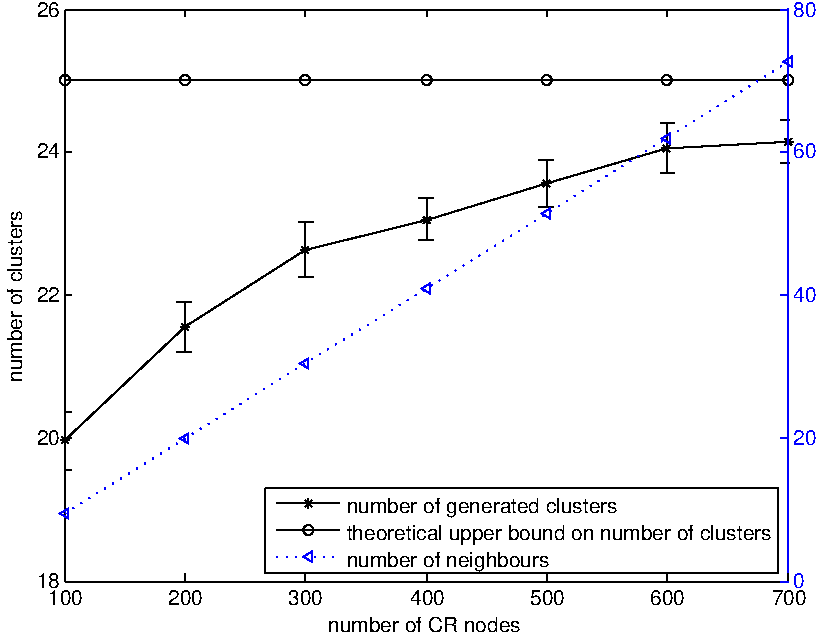
\includegraphics[width=0.67\linewidth]{number_clusters_upperBound.pdf}
  \caption{Number of clusters formed}
  \label{number_clusters_scale}
\end{figure}

Both the analysis and simulation show that with the increase of network density, the cluster size also increases.
In case of dense network where cluster size is large, there is substantial burden on cluster heads to manage the cluster members, which is a challenge for resource limited cluster heads.
As a result, certain measures are needed to prevent the network size to increase with the increasing network density.
This task falls on cluster head.
To control cluster size, cluster heads prune their cluster members if sizes are greater than the desired size $\delta$.
Given desired size as $\delta$, cluster head excludes members sequentially, whose absence leads to the maximum increase of common channels within the cluster.
This process ends when the size of resultant cluster is at most $\delta$ and at least one \gls{CCC} is available.
This procedure is similar with guaranteeing CCC available to be available in cluster, thus the algorithm is also given in Algorithm~\ref{alg_size_control_available_CCC}.


\begin{algorithm}               % enter the algorithm environment
\caption{CCC guarantee and cluster size control by cluster head}          % give the algorithm a caption
\label{alg_size_control_available_CCC}
\DontPrintSemicolon
\SetAlgoLined
\KwIn{Initial cluster formed, empty sets $\mathcal{T}_1, \mathcal{T}_1$}
\KwOut{cluster has at least CCC, and satisfies the requirement on cluster size}
\tcc*[r]{When available CCC is to be guaranteed, execute line 1, when cluster size control is conducted, execute line 2}
\textbf{while} $V_C =\emptyset$ \textbf{do}\\
\While{$|C|>\delta+1$}{
calculate $\lambda = \min_{i\in C, i\neq H_C}(|K_{H_C}\cap K_i|)$;\\
	\For{each $i\in C\setminus H_C $}{
	\If{$|V_{H_C}\cap V_i| ==\lambda$}{$\mathcal{T}_1\leftarrow i$}
	}
\eIf{$|\mathcal{T}_1|==1$}{delete node $i$ from $C$;\\break;}
{
calculate $\mu= \Max_{i\in \mathcal{T}_1}(|\cap_{j\in C\setminus i} V_j|-|\cap_{j\in C} V_j|)$;\\
	\For{each $i\in \mathcal{T}_1$}{
	\If{$|\cap_{j\in C\setminus i} V_j|-|\cap_{j\in C} V_j| ==\mu$}{$\mathcal{T}_2\leftarrow i$}
	}
\eIf{$|\mathcal{T}_2|==1$}{delete node $i$ from $C$;\\break;}
	{
	delete $i\in \mathcal{T}_2$, which has the highest ID;
	}
}
}
\end{algorithm}

%Figure~\ref{fig2} shows the clusters formed in the example in Figure~\ref{fig1} when the desired cluster size is 3. 

%Especially, it forster the connectivity between the clusters. It can do so, as the nodes with larger connectivity degree are not cluster heads but members. 
%As basin nodes have smaller $d_i$ compared with its cluster members, and many of the cluster members locate between the basin node and neighbor clusters,  %the bigger $d_i$ with bigger robustness of Social Connection, i.e, with bigger $d$ are located around cluster heads, 
%After clusters are formed, with aid of \textit{control channel rotation scheme} proposed in \cite{Lazos09}, intra and inter cluster communication is conducted and for each debable node (XXX Debatable nodes are not defined yet), the membership and channel availablity of the clusters concluding it is known. 


\begin{figure}[ht!]
  \centering
  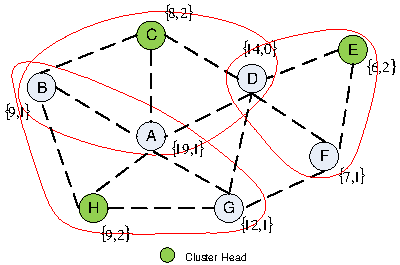
\includegraphics[width=0.6\linewidth]{figure2.pdf}
  \caption{Clusters formation after the first phase of ROSS. Some nodes remain debatable nodes after the first phase.}\label{fig2}
\end{figure}


\subsection{Phase II - Membership Clarification}
%\subsubsection*{Problem Description}
After applying ROSS phase I on the example in Figure~\ref{fig1}, we get the clusters shown in Figure~\ref{fig2}.
We notice there are several nodes, \ie $A, B, D$, are included into more than one cluster. 
We refer these nodes as \textit{debatable nodes} as their cluster affiliations are not clear, and the clusters which include debatable node $i$ are called \textit{claiming clusters} of node $i$, and are represented as $S_i$.  
Actually, debatable nodes extensively exist in CRN with larger scale.
Figure~\ref{percentage_overlapping_node} shows the percentage of debatable nodes increases with the scaling of CRN network.

Debatable nodes should be exclusively associated with one cluster and removed from the other claiming clusters, this procedure is called cluster membership clarification.
We will introduce the solution for cluster membership clarification in the following.

\begin{figure}[ht!]
  \centering
  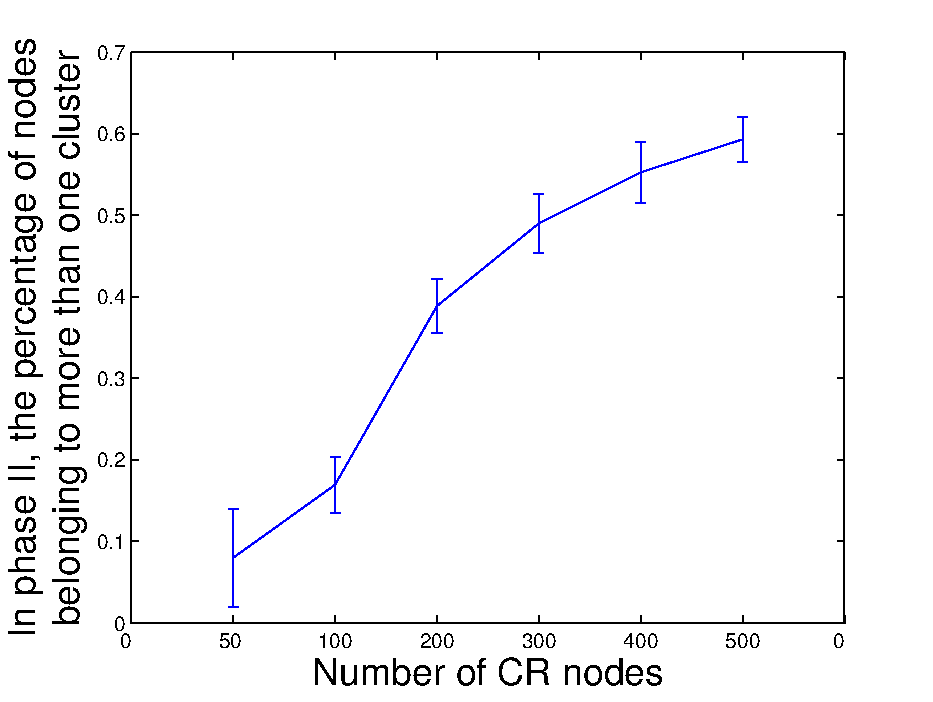
\includegraphics[width=0.6\linewidth]{percentage_overlapping_node.pdf}
  \caption{Clusters formation after the first phase of ROSS. Some nodes remain debatable nodes after the first phase.}\label{percentage_overlapping_node}
\end{figure}



%In the second phase of ROSS, debatable nodes will chose only one cluster to reside.

%In particular, the un-affiliation of one debatable nodes from a cluster increasing the set $K_C$ of ICCs of cluster $C$ (at the cost of potentially decreasing $R_C$, the set of OCCs).

%\newtheorem{observation}{Observation}
%\label{observation}
%\begin{observation}
%If the number of nodes within a cluster decreases, the number of common channels will increase or keep constant.
%\end{observation}
%
%\begin{proof}
%Contradiction, To be continued
%\end{proof}
%From observation 1 we know that the procedure of membership clarification will increase the set of common channels for some clusters and accordingly strengthen the robustness of intra connectivity. 

% % % % %	dependancy!
%An debatable node belongs to multiple clusters, and in the same time, it is possible that several debatable CR nodes locate within one same cluster. %Each debatable node tries to increase the sum of ICC of the clusters which it belong to. More specifically, 
%For a debatable node $i\in S_i$ after phase I, as to clarify its membership, it will choose one cluster $C\in S_i$ to stay and withdraw from the other clusters in $S_i$ with the consideration of increasing ICCs within $S_i$ by the largest margin. 

\subsubsection*{Distributed Greedy Algorithm}
%Debatable node $i$ is aware of all its claiming clusters in $S_i$. 
After Phase I, debatable nodes, \eg $i$ needs to decide which cluster $C\in S_i$ to stay, and leaves the others.
The principle for debatable node $i$ to choose one claiming cluster is to result in the greatest increase of common channels in all its claiming clusters.
%The set of available channels of one cluster are known by the debatable nodes which locate in that cluster. %this is finished 
Node $i$ communicates with all the cluster heads whose clusters are in $S_i$, and is aware of the vector of common channels of the claiming clusters, then $i$ is able to calculate how many more common channels in one certain claiming cluster if $i$ leaves that cluster.
Based on this calculation, $i$ decides in which claiming cluster to stay and leaves the other claiming clusters.
If there exists one cluster $C\in S_i$, by leaving from which the clusters in $S_i$ obtain the minimum increased common channels than leaving any other claiming clusters, then $i$ chooses to stay in cluster $C$.
When there comes a tie in terms of the increase of common channels among multiple claiming clusters, $i$ chooses to stay in the cluster whose cluster head shares more common channels with $i$.
In case there are multiple claiming clusters demonstrating the same on the aforementioned metrics, node $i$ chooses to stay in the smallest claiming cluster.
IDs of cluster heads will be used to break tie if the previous rule doesn't decide on the unique cluster to stay.

Algorithm for debatable node $i$ to decide which claiming cluster to stay is described as Algorithm~\ref{alg4}.
To conduct Algorithm~\ref{alg4}, debatable node $i$ needs to know the necessary information about its claiming clusters, \ie $V_C$, $V_{H_C}$, $|C|$,$C\in S_i$, which are respectively the set of available channels in $C$, the set of available channels on $C$' cluster head $H_C$, and $C$' cluster size.
Node $i$ decides which cluster to stay based on Algorithm~\ref{alg4}, then notifies all its claiming clusters, and retrieves the updated information of the necessary information $V_C$, $V_{H_C}$, $|C|$, where $C\in S_i$.

\begin{algorithm}               % enter the algorithm environment
\caption{Debatable node $i$ decides its affiliation, chooses one claiming cluster to stay and leaves all the other claiming clusters}          % give the algorithm a caption,  cluster to settle
\label{alg4}
\DontPrintSemicolon
\SetAlgoLined
\KwIn{all claiming clusters $C\in S_i$}
\KwOut{one cluster $C$}
calculate $\lambda = \Min_{C\in S_i}(|K_{C\setminus i}|-|K_C|)$;\\
define set $\mathcal{C}_1$;\\	
	\For{each $C\in S_i$}{ 
	\If{$|K_{C\setminus i}|-|K_C| ==\lambda$}{$\mathcal{C}_1\leftarrow C$}\tcc*[r]{metric is the increase of CCCs due to $i$' departing}
	}
\eIf{$|\mathcal{C}_1|==1$}{choose cluster $C$;\\break;}
{
calculate $\mu= \Max_{C\in \mathcal{C}_1}(V_{H_C}\cap V_i)$;\\
define set $\mathcal{C}_2$;\\	
	\For{each $C\in \mathcal{C}_1$}{
	\If{$V_{H_C}\cap V_i ==\mu$}{$\mathcal{C}_2\leftarrow C$}\tcc*[r]{metric is the number of common channels between $i$ and cluster head of demanding cluster}
	}
\eIf{$|\mathcal{C}_2|==1$}{choose cluster $C$;\\break;}
	{
	calculate $\nu=\min_{C\in \mathcal{C}_2}|C|$;\\
	define set $\mathcal{C}_3$;\\	
		\For{each $C\in \mathcal{C}_2$}{
		\If {$|C|==\nu$}{$\mathcal{C}_3\leftarrow C$}	\tcc*[r]{metric is cluster size}
		}
	\eIf{$|\mathcal{C}_3|==1$}{choose cluster $C$;\\break;}
		{choose the $C\in \mathcal{C}_3$, which has the highest ID;
		}
	}
}
Node $i$ notifies $H_C$ which is cluster head of $C$ of its affiliation decision, cluster $C$ then accepts it.

\end{algorithm}



This procedure raises the concern on infinite chain effect that debatable nodes update their choices based on other debatable nodes' choices, and never cease.
Assume debatable node $i$ locates in one cluster $C\in S_i$, and $C$ could have more than one debatable node except for $i$.
Let $i$ our of $C$'s debatable nodes to make decision on the cluster to stay first.
Then the choices of those debatable nodes except for $i$ change $C$'s membership, which possibly further triggers node $i$ to alter its previous decision.
%To maximize the increase of common channel in clusters in $S_j$, $j$ either stays in $C$, or leaves cluster $C$ and stay another cluster in $S_j$.
%$j$'s decision changes $C$'s membership, which will affect $i$'s decision.
%Assume $i$ makes decision before $j$ and chooses to stay in $C$, as which brings the most common channels in $i$' claiming clusters, and then it is $j$' turn to choose cluster.
%If $j$ leaves $C$, the smaller cluster $C$ will possibly make $i$ to leave it and join another cluster.
%and the choice of $j$ to stay in $C$ or not possibly changes $C$'s membership and  which potentially further triggers node $i$ to alter its previous decision. 
Thus, we must answer this question raised when implementing ROSS-DGA.
%, and if it converges, how good such a distributed scheme performs. 
In the following we show that the process of membership clarification can be converted to a congestion game, and a equilibrium state is reached after a finite number of best response updates.

\subsubsection*{Bridging ROSS-DGA with Congestion Game}
In this part, we illustrate that when debatable nodes decide on the exclusive clusters to stay, in particular, the 
To formulate the problem of membership clarification for the debatable nodes in the context of a game, we look at the problem from a different perspective. 
In the new perspective, the debatable nodes are regarded as isolated and don't belong to any cluster, which means the clusters they used to belong to become their neighbouring clusters. 
Then as to each debatable node, the previous problem to decide which clusters to leave becomes a new problem that which cluster to join.
In this new problem, debatable node $i$ (note now $i\notin S_i$) chooses one cluster $C$ out of $S_i$ to join if the decrement of common channels in cluster $C$ is the  %(among the clusters set $CS$, but now, each cluster $C\in CS$ does not conclude $i$) 
smallest in $S_i$, and the decrement of CCCs in cluster $C$ is $\sum_{C\in S_i}\Delta\vert K_C \vert=\sum_{C\in S_i}({\vert K_{C} \vert-\vert K_{C\cup i} \vert})$. %  $c'$ is the cluster after implementing the strategy, and $c$ is the original cluster.
The relation between debatable nodes and claiming clusters is shown in Figure~\ref{debatable_nodes_claiming_cluster}.
\begin{figure}[ht!]
  \centering
  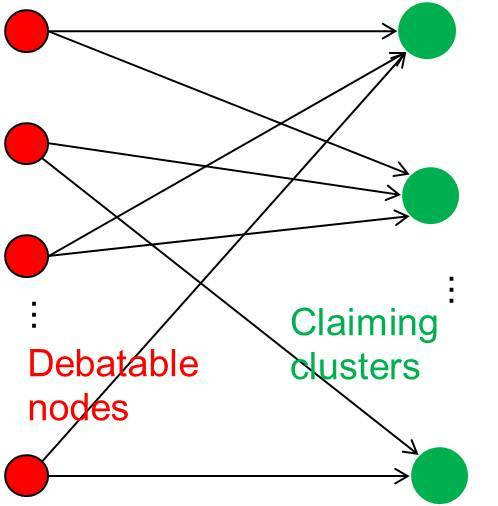
\includegraphics[width=0.30\linewidth]{singletongame.pdf}
  \caption{debatable nodes and claiming clusters}
  \label{debatable_nodes_claiming_cluster}
\end{figure}

In the following, the debatable nodes constitute the players, and the 
we show that the decision of debatable nodes to clarify their membership can be mapped to the behaviour of the players in a \textit{player-specific singleton congestion game} when proper cost function is given.

The game to be constructed can be represented by a 4-tuple $\Gamma=(\mathcal{P},\mathcal{R},(\sum_i)_{i \in \mathcal{N}},\Delta\vert K^i_C \vert)$, where elements in $\Gamma$ are given as below,
%To make the model of this game more clear, we make some change to our original problem. Previously, the nodes in overlapping areas belong to more than one cluster, and our scheme is to remove them out of some clusters to increase the set of common channels within the cluster form which the mode leave. In the new model, we assume all the nodes in overlapping nodes don't belong any cluster and the problem become into how do these nodes decide which cluster to join.

%The components of the game are listed as follows,

\begin{itemize}
%	\item $\mathcal{D}=\left\{1,\ldots,n\right\}$, the set of players (debatable nodes).
	\item $\mathcal{P}$, the set of players of the game, which are the debatable nodes after phase I in our clustering problem.
%	\item $\mathcal{R}=\left\{1,\ldots,m\right\}$, the set of resources which player can choose, which are all the clusters in our model.
	\item $\mathcal{R} = \cup S_i, i\in \mathcal{P}$, denotes the set of resources for players to choose, $S_i$ is the set of claiming clusters of node $i$. $\mathcal{R}$ is the set of claiming clusters after phase I in our clustering problem.
	\item As to the strategy space $\sum_i$ of player $i\in \mathcal{N}$, there is $\sum_i \subseteq 2^{\left[S_i\right]}$. As one debatable node is supposed to choose one claiming cluster in our problem, thus only one resource is allocated for $i$, accordingly this congestion game is a singleton game.
	%when $i$ makes decision, only one resource (one claiming cluster) from the allowed resources is allocated.
	
	%\item We denote by $\mathcal{S}=\left(\mathcal{S}_1,\ldots,\mathcal{S}_n\right)\in \sum_1\times \cdots\times\sum_n$ the state of game where player $i$ plays strategy $\mathcal{S}_i\in \Sigma_i$.
	
	\item %For the clusters which are possible destination of debatable nodes, the decrement of common channels caused by different debatable node' join can be different because of the heterogeneity of channel availability within itself and on the debatable nodes. %furthermore, the sequence of debatable node's join can also alter the decrement. 
	The utility (cost) function $f(C)$ of resource $C\in R$, (or to say $f(r)$ of resource $r \in \mathcal{R}$) is $\Delta\vert K^i_C \vert$ which represents the decrement of CCCs in cluster $C$ caused by debatable node $i$' joining in it.
	As to cluster $C\in S_i$, the decrement of CCCs caused by enrolment of debatable nodes is $\sum_{i:C\in S_i, i\rightarrow C} \Delta\vert K^i_C \vert$. 
$i\rightarrow C$ means $i$ joins in cluster $C$.
Obviously this function is non-decreasing with respect to the number of nodes joining in cluster $C$.
	
The utility function is not purely decided by the number of players (debatable nodes) as that in a canonical congestion game, as in this game the channel availability on debatable nodes is different.
Given two same sized groups of debatable nodes, when the nodes are not completely the same (neither are the channel availabilities on these nodes), the cost happened on one claiming cluster could be different if the two groups of debatable nodes join in that cluster respectively.
%In a canonical congestion game, the cost (or pay off) is function of only the number of players occupying the resource, and is mono-
%In this new game, the cost function 
Hence, this game is called player specific.
In this game, every player greedily updates its strategy (choosing one claiming cluster to join) if joining in a different claiming cluster minimizes the decrement of CCCs $\sum_{i:C\in S_i} \Delta\vert K^i_C \vert$, player's strategy in the game is exactly the same with the behaviour of debatable node in membership clarification phase, which is described by Algorithm~\ref{alg4}.


%	\item The Rosenthal's potential function \cite{Rosenthal} of this congestion game is given by:
%	\begin{equation*}
%	\phi(S)=\sum_{C\in\mathcal{R}} \sum_{i:C\in S_i} \Delta\vert K^i_C \vert   	
%   	%\sum_{i=1}^N \Delta^{i}_{p}(S)=\sum_{i=1}^N \sum_{r\in S_i}\Delta^{i}_{r}(t)	
%  	% \Delta =\sum_{i=1}^N w_i (x_i - \bar{x})^2 .
%	\end{equation*}
%All the players in this game greedily update their strategy to minimize the potential function (congestion), this process is exactly the same with the network behaviour under \textit{Distributed Greedy Algorithm}. 

%	\item It is an asymmetric game because the sets of strategies shared by different players are different.
%	\item The total cost is: 
%\begin{equation*}
%   \sum_{i=1}^N \Delta^{i}_{p}(S)=\sum_{i=1}^N \sum_{p\in s_i} \Delta^{i}_{p}(n_p(S))
%  % \Delta =\sum_{i=1}^N w_i (x_i - \bar{x})^2 .
%\end{equation*}

%This is the global objective we want to minimize.
\end{itemize}

%Singleton congestion game is a special type of matroid game~\cite{Milchtaich1996111,}. 
%It is known that player-specific matroid congestion game admit pure equilibrium, 

As to singleton congestion game, there exists pure equilibria which can be reached with greedy update~\cite{Ackermann06purenash}.


%and the number of steps towards \textit{Nash Equilibrium} is upper-bounded\footnote{Here we present this with modifying the original conclusion in \cite{Ackermann06purenash} according to our model.} by $ n^2\cdot m $. In our context, $n$ is the number of debatable nodes, $m$ is number of clusters in CRN, %$rk(\Gamma)$ of the matroid  is the cardinality of the maximal independent sets, which is 1 in the case of singleton game, 
%so the total time complexity to achieve the \textit{Nash Equilibrium} using greedy approach is 	.
%%(XXX Just mention after this complexity result the relationship to the system mdeol XX)
%This is upper-bounded (in the worst case) by $O(\vert I\vert^3)$. 
Based on above model and analysis, phase II converges is Algorithm~\ref{alg4} is run by debatable nodes. 
%Although the game version of DGA can achieve \textit{Nash Equilibrium}, the whole scheme can possibly obtain sub-optimal result.    %, furthermore,this stable state is a local minimum of the global decrement function.
%\todo[inline]{The number of steps, or the upper bound of steps in convergence needs a formal proof}

\subsubsection*{Distributed Fast Algorithm (DFA)}
The complexity of DGA is quite large recalling that the formation of clusters takes at most $|I|$. Here we propose a faster algorithm DFA which is especially suitable for CRN where channel availability might change dynamically and re-clustering is possible. %Note that the algorithm is based on the problem description of phase II. 
In DFA, each debatable node executes only one iteration of Algorithm~\ref{alg4} (by setting 'the current value' in Line 14 to zero). Every cluster includes all its debatable nodes, thus the membership is static and debatable nodes can make decisions simultaneously without considering the change of membership of its claiming clusters. For example, for node $A$ in Figure \ref{fig2}, the membership of cluster $C_C, C_H\in S_A$ are $\{A,B,C,D\}$ and $\{A,B,H,G\}$ respectively. 

The two possible strategies of node $A$'s clarification is illustrated in Figure \ref{fig3}. In Figure \ref{AinC}, node $A$ staying in $C_C$ and leaving $C_H$ brings 2 more CCC in $S_A$, as it is more than that brought by another strategy showed in \ref{AinH}, $A$'s membership is clear. After the decisions made similarly by the other debatable nodes $B$ and $D$, the final clusters formed are shown in Figure~\ref{fig4}.

%Using DFA in phase II, the time complexity is decreased drastically to 1. Thus, the total complexity of ROSS-DFA is $|I|$, while, ROSS-DGA's complexity is $|I|^3$ in the worst case.


\begin{figure}[ht!]
\centering
\subfigure[Node A stays in cluster $C_C$, quits $C_H$, $\Delta\vert K_{C_C}\vert+\Delta\vert K_{C_H}\vert=2$]{
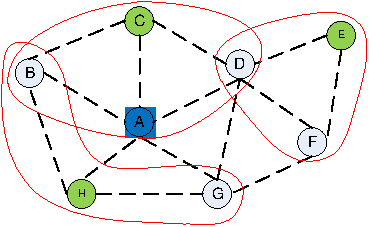
\includegraphics[width=0.435\linewidth]{figure4AinC.pdf}
\label{AinC}
}
\subfigure[Node A stays in cluster $C_H$, quits $C_C$, $\Delta\vert K_{C_C}\vert+\Delta\vert K_{C_H}\vert=1$]{
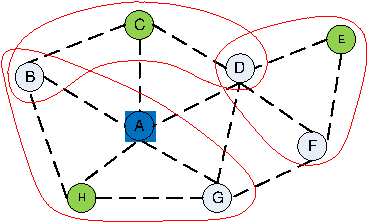
\includegraphics[width=0.435\linewidth]{figure4AinH.pdf}
\label{AinH}
}
\caption[]{Membership clarification: possible cluster formations decided by node A's different choices} %\subref{node A in $C_C$}, \subref{node A in $C_H$}}
\label{fig3}
\end{figure}

\begin{comment}
As an example, when node A comes to decide which cluster to stay, the memberships of relevant clusters, like $C_C$ and $C_H$, are $\{C,B,D,A\}$ and $\{H,B,G,A\}$ respectively. Before the other two debatable nodes B and D making their belonging clear, cluster $C_C$ and $C_H$ have them in the same time. So node A can decide which cluster to belong to without considering other debatable nodes' action. There are two strategies for node A, which is illustrated in Figure \ref{fig3}. Because staying in cluster $C_C$ brings in more common channels within relevant clusters, node A finally choose cluster $C_C$ to stay and caveat from cluster $C_H$. The membership of $C_H$ is updated in the same time. Node B and D undertake the same process and the clusters are formed finally as Figure \ref{fig4} shows.

Because debatable nodes can conduct membership clarification abased on static membership information of relevant clusters, thus no iteration happens in this process. The time complexity of this algorithm is only decided by the number of debatable nodes, which is maximal $O(\vert I\vert)$. 

As an example, when node A comes to decide which cluster to stay, the memberships of relevant clusters, like $C_C$ and $C_H$, are $\{C,B,D,A\}$ and $\{H,B,G,A\}$ respectively. Before the other two debatable nodes B and D making their belonging clear, cluster $C_C$ and $C_H$ have them in the same time. So node A can decide which cluster to belong to without considering other debatable nodes' action. Figure \ref{AinC}. Because staying in cluster $C_C$ brings in more common channels within relevant clusters, node A finally choose cluster $C_C$ to stay and retreat from cluster $C_H$. The membership of $C_H$ is updated in the same time. Node B and D undertake the same process and the clusters are formed finally as Figure \ref{fig4} shows.
\end{comment}


\begin{figure}[ht!]
  \centering
  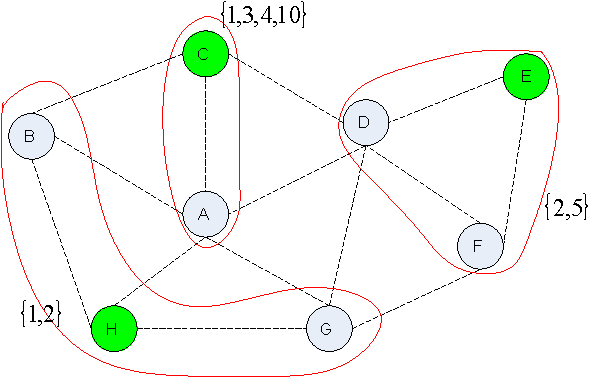
\includegraphics[width=0.5\linewidth]{final_clustering_ross.pdf}
  \caption{Final formation of clusters, common channels for each cluster is shown.}
  \label{fig4}
\end{figure}


\newpage
\section{Centralized Clustering Scheme}
\label{centralized_scheme}

%paper given by james is useful which provides a survey from the perspective of wsn!


%\todo[inline]{check}
The centralized clustering scheme aims to form clusters with certain sizes, meanwhile the total number of common channels of all clusters is maximized.
In the following, we refer this problem as \textit{centralized clustering} for short, and the problem definition is as follows, 


\begin{mydef}
\label{def_centralized_clustering}
\textit{Centralized clustering in CRN.}

Given a cognitive radio network $\mathcal{N}$ where nodes are indexed from 1 to $N$ sequentially.
Based on certain correlation, certain secondary users constitute one cluster $C$.
$1\leq |C| \leqslant k$ where $|C|$ is size of cluster $C$ and $k$ is positive integer.
We name the collection of such clusters as $\mathcal{S}=\{C_1, C_2,\ldots,C_{|\mathcal{S}|}\}$ (the subscript $i$ is the unique index of cluster in $\mathcal{S}$, not the ID of cluster head of relevant cluster), $\mathcal{S}$ has following properties: $\bigcup_{1\leq i \leq l} C_i = N$ and $V_{C_i}\neq \emptyset$ for any $i$ which satisfies $1\leq i \leq l$.

Following condition distinguish the centralized clustering problem discussed in this thesis.
The number of common channels is denoted as $f$ which is $|V_{C}|$ if $|V_{C}|>1$, and $f=0$ if $|V_{C}|=1$.
The question of this problem is to find a subcollection $\mathcal{S}' \subseteq \mathcal{S}$, so that $\bigcup_{C_j\in \mathcal{S}'} C_j = N$, and $C_j'\cap C_j =\emptyset$ for $C_j', C_j\in \mathcal{S}'$, so that $\sum_{C\in \mathcal{S}'} f$ is maximized.
% when $|C|>1$, and $f(\cdot)=0$ when $|C|=1$.
%As to $f(\cdot):z\rightarrow z$, under this problem setting, if only number of common channels are given consideration, only singleton clusters will be preferred, which contradicts to our goal of clustering CR nodes together, thus we choose $f(\cdot)= |V_{C}|\cdot |C|$, the product of number of common channels and cluster size.
The decision version of centralized clustering in CRN is to ask whether exist $\mathcal{S}'\subseteq \mathcal{S}$, so that $\sum_{C\in \mathcal{S}'} f \geqslant \lambda$ where $\lambda$ is a real number.% in stead of to maximize $\sum_{C\in \mathcal{S}'} f$.
\end{mydef}


%The decision version of \textit{weighted exact cover problem}: 
%Given an universe $U$, and collection $S=\{s_1, s_2, \ldots, s_m\}$ where each subset $s_i\subseteq U$ and is given a weight $w_i$, whether there exists a collection of subsets $\mathcal{C}$ and constant number $\lambda$, so that the union of $\mathcal{C}$ equals to $U$, $s_j\cap s_{j'} = \emptyset$ for different $j$ and $j'\in \{1,2,\ldots, m\}$, and $\sum_{i\in J} w_i \geq \lambda$.

In the following part of this section, we will discuss the complexity of centralized clustering problem and provide solution for it.
We put the definition of weighted k-set packing problem here as it will be used in the analysis on the complexity of our problem.

\begin{mydef}
\label{def_kset_packing}
\textit{Weighted k-set packing.} 

Given a set $\mathcal{G}$ which contains finite number of positive integers, and a collection of set $\mathcal{Q}=\{s_1,s_2,\cdots,s_m\}$, where for each element $s_r, 1\leq r \leq m$, there is $s_r\subseteq \mathcal{G}$, $ 1\leq|s_r| \leq k$, and $s_r$ has an associated weight which is positive real number.
The question is whether exists a collection $\mathcal{S}\subseteq \mathcal{Q}$, where $\mathcal{S}$ contains only disjoint sets and the total weight of sets in $\mathcal{S}$ is greater than $\lambda$.
Weighted k-set packing is NP-hard when $k\geqslant 3$.~\cite{Computers_a_Intractability}
\end{mydef}

\begin{theorem}
\label{theorem1}
CRN clustering problem is NP-hard, when the maximum size of clusters $k\geqslant 3$.
%Assume a CRN can be represented by a connected graph, and there is at least one common channel between any pair of neighbours, then forming at least two CR nodes into one cluster is NP-complete.
\end{theorem}

\begin{proof}
To see centralized clustering problem is NP-hard, we reduce the NP-hard problem \textit{weighted k-set packing} to it.
%, which means centralized clustering in CRN problem is as hard as weighted k-set packing to be solved.

To complete the reduction, we need to conduct following two steps:
\begin{itemize}
\item step 1: Show there exists a polynomial algorithm $\sigma$, by which any instance (\eg $\mathcal{S}$) of a weighted k-set packing can be transformed to instance $\sigma(\mathcal{S})$ for centralized clustering.
\item step 2: Show that $\mathcal{S}$ is a \textit{yes} instance of weighted k-set packing if and only if $\sigma(\mathcal{S})$ is an \textit{yes} instance for CRN clustering problem.
\end{itemize}

We continue using the notation introduced in problem definition.
Let set $\mathcal{G}$ contains $N$ positive integer numbers which are indexed from 1 to $N$ sequentially.
Assume one instance $\mathcal{S}$ of weighted k-set packing is a collection of disjoint sets $\mathcal{Q} = \{s_1, s_2,\cdots s_m\}$, each set is composed by certain amount of elements in $\mathcal{G}$.
$\omega$ indicates the weight for each set $s$, $\omega:\mathcal{S}\rightarrow \mathbb{Z}^{+}$.
%As the number of common channel of clusters is always integer
%give new weight to them in following way



The polynomial algorithm $\sigma$ consists of three transformations.
\begin{itemize}
\item In the first transformation, for each set $s_i$ of instance $\mathcal{S}$, the elements are duplicated, for instance, given $s_i=\{1, 4, 6\}$, the dummy set $s_i'$ is $\{1,1,4,4,6,6\}$.
By doing this, we obtain the dummy sets and constitute the dummy instance $\mathcal{S}'$ based on $\mathcal{S}$.
The purpose of this transformation is to eliminate the single element set in $\mathcal{S}$.
The weight of set is unchanged after this transformation, \ie $\omega(s_i)=\omega(s_i')$.
After this transmission, there is no set with only one element.
This transformation requires $\sum_{s_i \in \mathcal{S}} |s_i|$ steps.
\item In the immediate following second transformation, we transform the dummy instance $\mathcal{S}'$ to an instance for CRN clustering problem.
Given an instance $\mathcal{S}'$, we retrieve all the elements which appear in it, and map each of those elements into one CR node, \ie each integer corresponds to one CR node, particularly, that integer becomes the CR node's ID.
As to duplicated elements, we also map them into a CR node, thus there exist CR nodes with the same ID.
As a result, these CR nodes constitute a collection of CR nodes, but note that they have not constituted one CRN yet as there are not connections drawn among them.
Connections in CRN under this context is decided by physical conditions, which says the corresponding CR nodes have common channels and close enough to communicate with each other.
This transformation requires $2\cdot\sum_{s_i \in \mathcal{S}} |s_i|$ steps.
%We further assume that all CR nodes locate in a way that any two pair of nodes has potential to be connected if their IDs are in the same set in $\mathcal{S}$, the instance for weighted k-set packing.
\item Mere isolated nodes don't constitute network, thus we add connections in CRN based on the sets in $\mathcal{S}'$ sequentially.
For each set $s'\in \mathcal{S}'$, we add connection between two CR nodes if their IDs are in $s'$.
There is also connection between the CR node and its dummy node.
The number of common channels of the CR nodes equals to the weight of set $s'$.
No connection exists between two CR nodes if their IDs don't appear in one set in $\mathcal{Q}$.
Afterwards, the CR node whose ID doesn't appear in any set in $\mathcal{S'}$ becomes single node clusters, according to the definition of clustering problem in CRN, the number of common channels is 0.
This procedure requires $\sum_{s_i' \in \mathcal{S}'} |s_i|$ steps to map sets in $\mathcal{S}'$ into CRN and connections, and at most $N$ steps to complement the single node clusters in CRN.

The number of common channels of cluster $f$ is non-decreasing function of cluster size, while, the weight of set in weighted k-set packing problem doesn't have this property.
In weighted k-set packing, the weight of a set with smaller size could be larger than a set with more elements.
But this difference doesn't hinder the transformation and we use an example to explain.
%There is one situation deserving extra explanation in the second transformation, we adopt one example to discuss it.
Assume two sets in $\mathcal{S}$ are $s_1=\{1,2\}$ and $s_2=\{1,2,3,4\}$, their weights are 3 and 5 respectively.
Their dummy sets are $s_1'=\{1,1,2,2\}$ and $s_2'=\{1,1,2,2,3,3,4,4\}$ and their new weights are 3 and 5 as before.
The connections mapped to CRN are contradictory to reality, as the number of common channels of CR node group $\{1,1,2,2\}$ can only be smaller than that of $\{1,1,2,2,3,3,4,4\}$.
We let this contradiction in the process of mapping happen because it will be eliminated later: no matter one instance $\mathcal{S}$ for weighted k-set packing results in \textit{yes} or \textit{no}, at most only one set of $s_1'$ and $s_2'$ is chosen, then we can safely delete the connections based on the deleted set from the CRN, and the contradiction is eliminated.
\end{itemize}






We have crossed the hurdle of finding one polynomial algorithm $\sigma$ to transform instance of weighted k-set packing to an instance for clustering in CRN.
Now we look into the step 2 in reduction.

When the instance $\mathcal{S}$ for weighted k-set packing contains one solution, \ie there is a group of sets in $\mathcal{S}$, whose sum weights is greater than $\lambda$, then in the CRN which is mapped from $\mathcal{S}'$, the sum number of common channels of the clusters which correspond to the selected sets in $\mathcal{S}$ and $\mathcal{S}'$, is greater than $\lambda$.

When there is no solution out of set $\mathcal{G}$ for weighted k-set packing, let's assume the maximum sum of weights of all instances is $\sum_{s_i\in \mathcal{S}}\omega(s_i)=\delta < \lambda$. 
The dummy set of each $s_i\in \mathcal{S}$ is mapped to cluster of CR nodes.
Definition of CRN clustering regulates that the number of common channels is 0 when the cluster has only one node.
As to $|s_i|=1$, the mapped cluster has two nodes, with one of them is the dummy CR node.
Then number of common channels is on longer 0 but equals to the weight of corresponding set $s_i$.
%Meanwhile, the number of common channels of all the other single node cluster is 0.
Then the sum number of common channels of the clusters in CRN is $\delta < \lambda$, thus, there is no clustering solution for the mapped CRN.

After proving weighted k-set packing can be reduced to centralized clustering in CRN, we can say the latter problem is NP-hard.
\end{proof}


\subsection{The Optimization Problem}

%Exact cover problem can be solved with Knuth's Algorithm X~\cite{dancingLinks_Knuth} as it finds out all the instances of exact cover, then we can choose the one with the biggest sum of weights. 
As there is no efficient algorithm to solve clustering problem in CRN, we adopt binary linear programming to solve the problem.
Note that binary linear programming is in NP-complete.

%This example indicates the chose of $\mathcal{C}$ plays an important role on the resultant clustering strategy.
%Meanwhile, it provide a chance to constrain the cluster size by putting groups with desired sizes into $\mathcal{C}$.

%the maximum size of $S$ is the \textit{Bell number} of $N$, and $S$ contains the conditions cluster .
%In this case, the resultant $\mathcal{C}$ is composed with all the singleton clusters, \ie, the cluster which contains one node, and the objective is -38.

%it is possible that there doesn't exist combination of clusters with the same cluster size.
%We thus list all possible clusters whose sizes are from 2 to one certain number \footnote{this number of decided by the density of CR network, along with the occupation of PUs. We set this number as cluster size of the biggest cluster ever appears when conducting distributed schemes.}, and check each combination of clusters to find the best covering of network on the aspect of number of ICCs per cluster.
%The complexity of computation is thus \bigO$(N^\delta)$, $\delta$ is the preferred cluster size.

%The global optimal clustering scheme with respect to the number of common channels is investigated to show the gap with the distributed schemes.


%We apply this centralized scheme on a network with network size $N$ and cluster size $\delta$.
%There is $N\mod \delta=0$, and the expected number of clusters is $C = N/\delta$.
%These tailored parameters don't harm the validity of the performance gap between the two schemes.

Given a CRN $N$ and desired cluster size $\delta$, we get a collection of clusters $G$, where clusters satisfy the conditions of clusters in Section~\ref{sec:model}, and the sizes of clusters are $1,2,\ldots,\delta$.
Note that the legitimate clusters include the singleton ones, which guarantees the partition of any network is feasible.
With $n=|N|,g=|G|$, we construct a $g\times n$ matrix $Q_{g\text{x}n}$. 
Each element $q_{ij}= |k_{C_i}|$ if $j\in C_i$, and $q_{ij}= 0$ if $j\notin C_i$.
In other words, Each non-zero element $q_{ij}$ denotes the number of common channel of the cluster $i$ where node $j$ resides.

\begin{figure}[ht!]
\centering
Q = \bordermatrix{~ 		& 1 	& 2 	& 3 	& \cdots & j & \cdots	& n-1 	& n	\cr
                  1 	& k_{1} 	& k_{1} 	& 0 	& \cdots & \cdots &\cdots	& 0 	& 0	\cr
                  2 	& k_{2} 	& 0 	& k_{2} 	& \cdots & \cdots & \cdots 	& 0 	& 0	\cr
				\vdots  	&\vdots & 	 	& 		&  \vdots		& 		& \vdots \cr
				i 	& 0 	& k_{i} 	& 0 	& \cdots  & \cdots & \cdots 	& k_{i} 	& 0	\cr
				\vdots  	&\vdots & 	 	& 		&  \vdots & \cdots & \cdots 		& 		& \vdots \cr
				\vdots 	& \vdots  	& 0 	& 0 	& \cdots & \cdots & \cdots 	& k_{i'} 	& 0	\cr
				g  	& k_{g} & 	 	& 		&  \vdots	& \cdots & \cdots& 	& 		& \vdots \cr}	
\caption{Matrix Q, }
\label{xx}
\end{figure}

We also have one $G\times N$ binary matrix $X$, the element of the matrix is binary variable $x_{ij},i=1, \ldots, G, j=1, \ldots, N$.
$x_{ij}=1$ denotes cluster $i$ is one partition chosen by the clustering scheme, $x_{ij}=0$ means this partition is not adopted.
\begin{equation}
\begin{aligned}
     &\min\limits_{x_{ij}} && \Sigma_{j=1}^g\Sigma_{i=1}^n (-x_{ij}q_{ij} + w_i*\texttt{cost($\delta$)}) \\
     &\text{subject to}   && \Sigma_{i=1}^g x_{ij} = 1,  j=1, \ldots, n \\
   &&& \Sigma_{j=1}^n x_{ij} = \delta*(1-w_i), j=1, \ldots, g \\
   &&& \text{$x_{ij}$ and $w_j$ are binary variables.}\\
   &&& i\in \{1,2, \cdots g\}, \hspace{0.3cm} j\in \{1,2,\cdots n\}
\notag
\end{aligned}
\end{equation}
As the resultant clusters are with certain desired sizes, we try to maximize the sum of products of cluster size and number of common channels in the objective function.
%The first item of the objective function is the sum of products of cluster size and number of common channels per cluster.
%When only this item is applied in the objective function, it is obvious to see that single node cluster strategy is the solution, hence we add the second item to control the cluster size.
The second item of objective function denotes the \textit{punishment} for choosing the cluster whose size is not $\delta$.
We design $\texttt{cost($\delta$)}$ as follows,

$$
\texttt{cost($\delta$)} = \left\{ \begin{array}{rl}
0 &\mbox{ if $|C_i|=\delta$} \\
\alpha_1 &\mbox{if $|C_i|=\delta-1$} \\
\alpha_2 &\mbox{if $|C_i|=\delta-2$} \\
\dots
\end{array} \right.
$$
where $\alpha_i>0$ and increases with $i$ getting larger.
Choice of $\alpha_i$ affects the resultant clusters.
%For instance, when the desired cluster size is $\delta$, if $x_ij=1$ and $|C_i|=\delta$, the 

Constraint 3.2 restricts that node $j$ resides in exactly one cluster. %, or resides in a single node cluster ($\Sigma_{i=1}^G x_{ij} < 1$). 
In constraint 3.3, $w_j$ is an auxiliary binary variable, $w_j=0$ denotes cluster $j$ is chosen in the solution.
When $w_i=1$, $i$th cluster is not chosen according to constrain 3.3, then the objective function suffers certain \textit{loss}.
%The constant $cost(\delta)$ is between 0 and $min(q_{ij}), i=1, \ldots, N, j=1, \ldots, G$.







%\begin{figure}[ht!]
%\centering
%\includegraphics[width=0.45\linewidth]{example.JPG}
%\caption{Example of Matrix Q in a 6-node network, cluster size is set as 2}
%\label{xx}
%\end{figure}

%\begin{figure}[ht!]
%  \centering
%  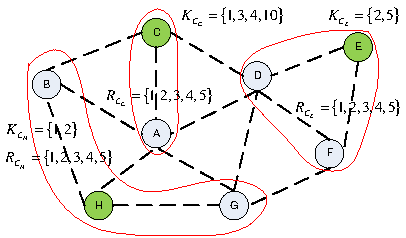
\includegraphics[width=0.5\linewidth]{figure5final.pdf}
%  \caption{Final cluster formation.}
%  \label{fig4}
%\end{figure}



This is a linear binary optimization problem, which is solved by function $bintprog$ provided in MATLAB.


Take CRN in Figure~\ref{fig1} for example.
As $|N|=8$, we let the cluster size $\delta$ to be either 2 or 3 so that the partition of network is possible.
A collection of clusters $G$ is built, where the clusters satisfy the conditions for cluster in Section~\ref{sec:model} and the sizes of clusters are 1, 2 and 3. 
$G=\{\{A\}, \{B\},\dots,\{B,C\},\{B,A\},\{B,H\},\cdots,\{B,A,C\},\{B,H,C\}, \{A,D,C\}$\\$,\cdots\}$, and $G=38$.
%Here we don't exhaustively list all the legitimate clusters with size 2 and 3.

The clustering result of binary linear programming is $\{\{D,E,F\},\{A,C,G\},\{H,G\}\}$, the number of common channels is $\{2,3,3\}$.
The solution from ROSS is $\newline \{\{B,H,G\},\{C,A\},\{D,E,F\}\}$, the number of common channels is $\{2,4,2\}$.
By applying SOC, the clustering result is $\{A,B,C,D,G\},\{E,F\},\{H\}$.

The final clusterings of the example CRN by SOC and linear programming are as follows,

\begin{figure}[ht]
\begin{center}
%\subfigure[ROSS]{\label{fig:final_clustering_ross}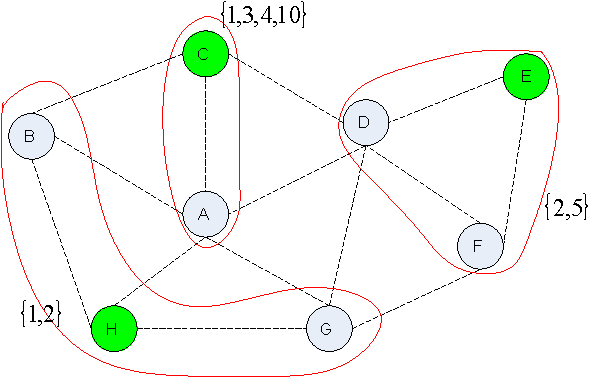
\includegraphics[width=0.3\textwidth]{final_clustering_ross}}
%
\subfigure[SOC]{\label{fig:final_clustering_soc}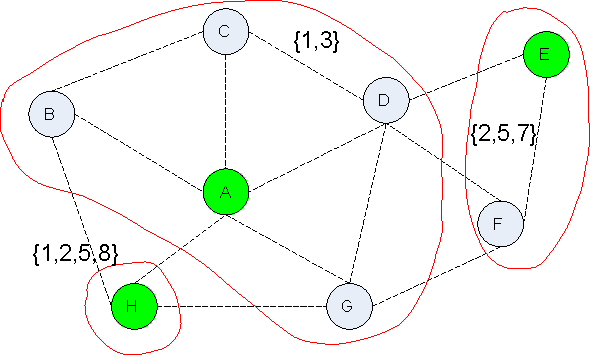
\includegraphics[width=0.45\textwidth]{final_clustering_soc}}
\subfigure[Linear programming]{\label{fig:final_clustering_LP}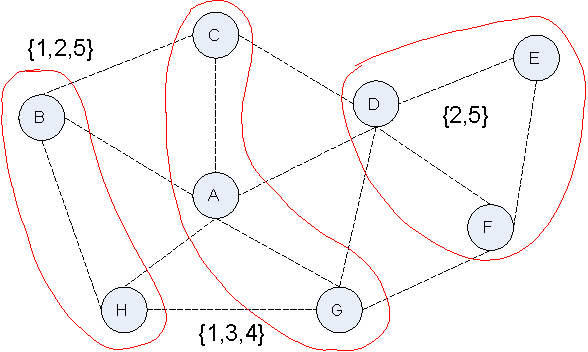
\includegraphics[width=0.45\textwidth]{final_clustering_LP}}
\end{center}
\caption{Final clustering of the example CRN}
\label{fig:final_clustering}
\end{figure}

As to the average number of common channel, the results of ROSS, LP and SOC are 2.66, 2.66, and 3 respectively. 
Note there is one singleton cluster $C_H$ generated.
When the singleton cluster $\{E\}$ is excluded, the average number of common channels of SOC drops to 2.5. 




\section{Performance Evaluation}
\label{performance}
In this section, we evaluate the performances of the two variants of ROSS, \ie ROSS-DGA and ROSS-DFA, besides, the cluster size control scheme is also evaluated when the desired cluster size is smaller than the average neighbourhood size.
We choose SOC as comparison scheme.
To the best of our knowledge, SOC~\cite{Lazos09} is the only work emphasizing on the robustness of clustering structure from all previous work on clustering in CRN. The authors of~\cite{Lazos09} compared SOC with other schemes based on the average number of common channels within each cluster, on which SOC outperforms other schemes by 50\%-100\%. This is because the schemes except for SOC are designed either for ad hoc network without consideration of channel availability~\cite{Basagni99}, or for CRN  but just considering basic connection among CR nodes~\cite{Zhao07}. Hence, we only compare the two versions of our scheme ROSS-DGA and ROSS-DFA with SOC to show the merits of ROSS, and also compare with the centralized scheme to see the gap with the global optima. 
We will investigate the following metrics:
\begin{itemize}
\item Average number of common channels per un-singleton cluster. 
\begin{itemize}
\item SOC adopts the average number of common channel over all clusters, \ie including the singleton clusters. As we try to look into the robustness of clusters of CRs, we exclude those singleton clusters.
\end{itemize}  

\item Number of unclustered CRs with moderate and vigorous intensity of PRs'activities.
\begin{itemize}
\item This is the straight forward metric on robustness of clusters.
We investigate how many clusters survives when we increase the intensity of PRs' activity.
\end{itemize}

\item Cluster sizes 
\begin{itemize}
\item Specific clusters size is pursued in many applications due to energy preservation and the system design ~\cite{clustering_globecom11}.
We will present the distribution of CRs residing in the formed clusters, and the number of generated clusters through multiple simulations.
\end{itemize}

\item Number of clusters	
\begin{itemize}
\item Homogeneous clusters size is pursued.
\end{itemize}

\item Amount of control messages involved.
\end{itemize}

The simulation is conducted with C++. 
Certain number of CRs and PUs are deployed within a squire whose edge is 100 m.
We adopt the round disk model to simulate transmission.
Transmission ranges of CR and PU are 10 and 30 respectively.
As to CRs, the CR node residing within another CR node's transmission range is seen as neighbour of that CR node.
If CR node locating within one PU's transmission range, the CR node is not allowed to use the channel which is being used by that PR.
The number of licensed channels in simulation is 10, each PU is operating on each channel with probability of 50\%.

There are two parts of simulation, in the first part, we investigate the gap between the distributed schemes with the centralized scheme.
As there is no polynomial time solution available to solve the centralized problem, we adopt a small network to compare the performances of the ROSS, SOC and the centralized solution.
In the second part, we increase the network scale and change network density to thoroughly compare the two distributed schemes.
\subsection{Centralized Schemes vs. Decentralized Schemes}
Coinciding with the system model in Section~\ref{sec:model}, 10 primary users and 20 CR users are dropped randomly (with uniform distribution) within some area of size $A^{2}$, where we set the transmission ranges of primary and CR users to $A/3$. There are $P=10$ available channels. 
With this setting, the average number of neighbours of one CR user is around 5.
Each primary user randomly occupies one channel, and CR users are assumed to be able to sense the existence of primary users and identify available channels.
When clustering scheme is executed, around 7 channels are available on each CR node.
All primary and CR users are assumed to be static during the process of clustering.
Performance results are averaged over 50 randomly generated topologies with equal parameters.
The desired cluster size is 3.
The confidence interval shown in figure corresponds to 95\% confidence level.

\subsubsection*{Number of Common Channels}
\label{ccc_20}
We first have a look at the average number of common channels per cluster, which is used in~\cite{LIU_TMC11_2} as the sole criterion for clustering robustness.
Figure~\ref{ccc_per_nonsingleton} shows the average number of common channel of non-singleton clusters, as the singleton clusters (in other words unclustered nodes) don't execute any functionalities of clusters, which are described in Section~\ref{intro}.
As to schemes, centralized schemes outperform distributed schemes on number of common channels.
SOC achieves the most number of CCC than variants of ROSS.
SOC is liable to group the neighbouring CRs which share the most abundant spectrum together, no matter how many of them are, thus the number of CCC of the formed clusters is higher, but this method leaves considerable number of CRs which have less spectrum not in any clusters.
As to variants of ROSS, the procedure of debatable nodes greedily looking for better affiliation improves the number of CCC, thus ROSS-DGA with and without size control outperform ROSS-DFA and its size control version respectively.
We also notice that, the size control feature doesn't affect the number of CCC for both ROSS-DGA and ROSS-DFA.


\begin{figure}[ht!]
  \centering
  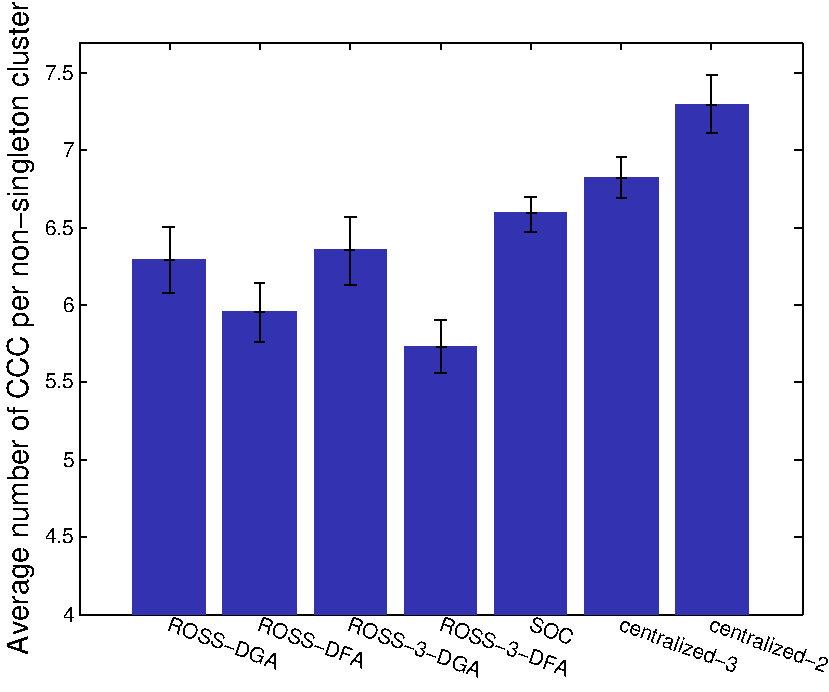
\includegraphics[width=0.65\linewidth]{ccc_20.pdf}
  \caption{Number of common channels for non-singleton clusters, the numbers in the names of schemes annotate the desired cluster size.}
  \label{ccc_per_nonsingleton}
\end{figure}

\subsubsection*{Survival Rate of Clusters with Increasing Primary Users}
We investigate the robustness of the formed clusters when they co-exist with varying intensity of PRs' activities.
After the clusters are formed under the influence of the initial 10 PRs, extra 100 PRs are sequentially added into the network.
The transmission range and channel occupancy of the new PU is the same with the previous ones, \ie transmission range is $A/3$, and one channel out of 10 is randomly chosen to operate.
As to one cluster, if there is no common channels available for all members because of the new added PRs, the cluster destroyed, and the former cluster member CRs become unclustered CRs.

Figure~\ref{singleton_clusters} shows the number of unclustered CRs with the increase of PRs, which indicates the vulnerability of clusters under varying surrounding of licensed spectrum.


We obtain three conclusions corresponding to three comparisons shown in this figure,
\begin{itemize}
\item Centralized scheme with cluster size of 2 produces the most robust clusters, and SOC results in the most vulnerable clusters.
Centralized scheme with cluster size of 3 achieves less unclustered CRs than variants of ROSS when the number of PRs is 10$\sim$30, when number of PUs is 30$\sim$60, same amount of unclustered CRs are generated with variants of ROSS.
When there are 75 and more new PRs, centralized scheme with cluster size of 3 results in more unclustered CR nodes than variants of ROSS.
Size control feature makes both ROSS-DGA and ROSS-DFA outperform themselves without size control when number of new PRs is greater than 50.

The reason that centralized scheme with cluster size of 3 does not completely excel variants of ROSS is due to the favourable achievement of it: the uniformly sized clusters.
As distributed schemes, variants of ROSS generate considerable amount of smaller clusters which are more likely to survive when PRs' activities become intense.
The comparison on cluster sizes will be given in details in~\ref{cluster_size}.

\item ROSS with size control is better than the other two distributed schemes.
The size control decreases the clusters size and makes the clusters more robust when under PRs' activity.

\item Greedy algorithm improves survival rate. 
ROSS-DGA improves the survival rate of ROSS-DFA, so does ROSS-DGA with size control against ROSS-DFA with size control.
This comply with the observation on number of CCC in section~\ref{ccc_20}.
As the debatable CRs greedily update their affiliation with demanding clusters, and the metric for updating is the maximum increase of CCCs of the demanding clusters, the average number of common channels is improved (shown in Figure~\ref{ccc_per_nonsingleton}), then the robustness of clusters is enhanced. 
Meanwhile, sizes of more clusters become smaller also contributes more robustness.

\end{itemize}

\begin{figure}[ht!]
  \centering
  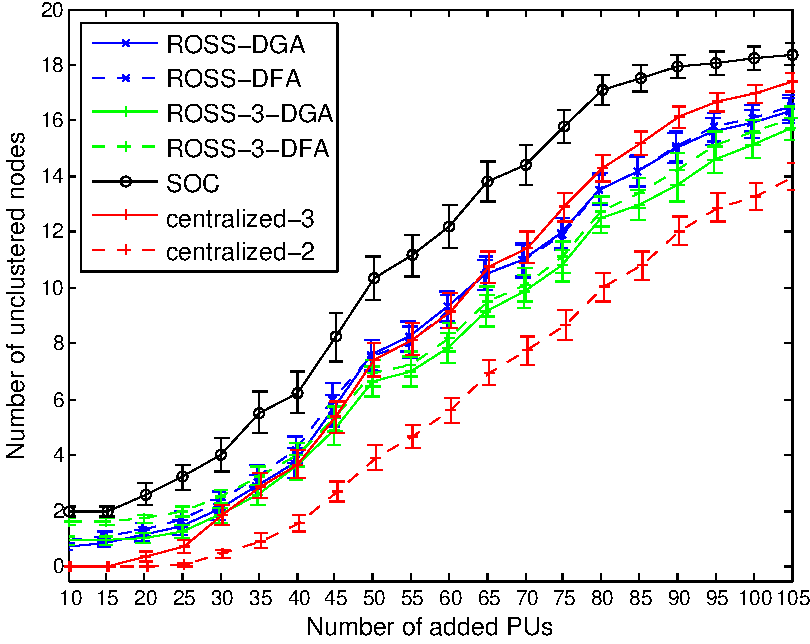
\includegraphics[width=0.7\linewidth]{survival_rate_20.pdf}
  \caption{Number of CRs which are not included in any clusters}
  \label{singleton_clusters}
\end{figure}

%\begin{figure}[ht!]
%  \centering
%  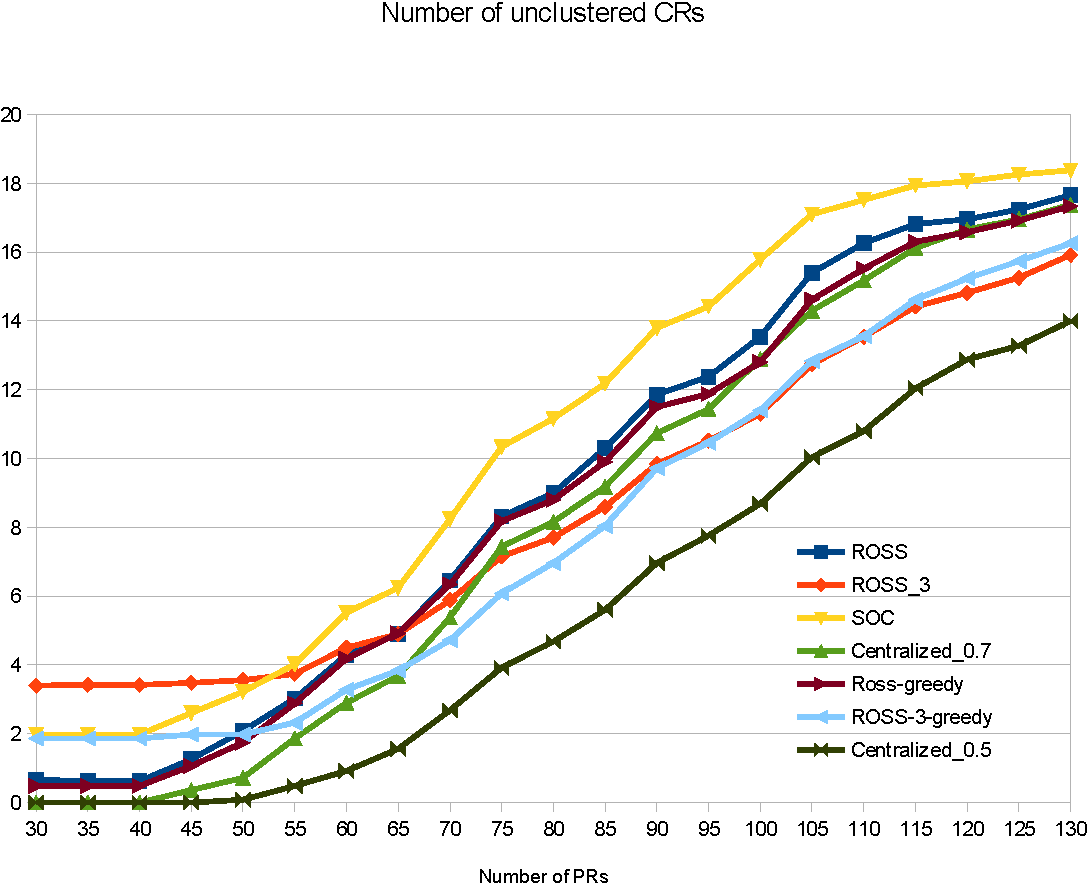
\includegraphics[width=0.5\linewidth]{singleton_clusters.pdf}
%  \caption{Comparison between Rocsi and centralized scheme on non-singleton clusters}
%  \label{singleton_clusters2}
%\end{figure}


\subsubsection*{Cluster Size Control}
\label{cluster_size}
\begin{figure}[ht!]
  \centering
  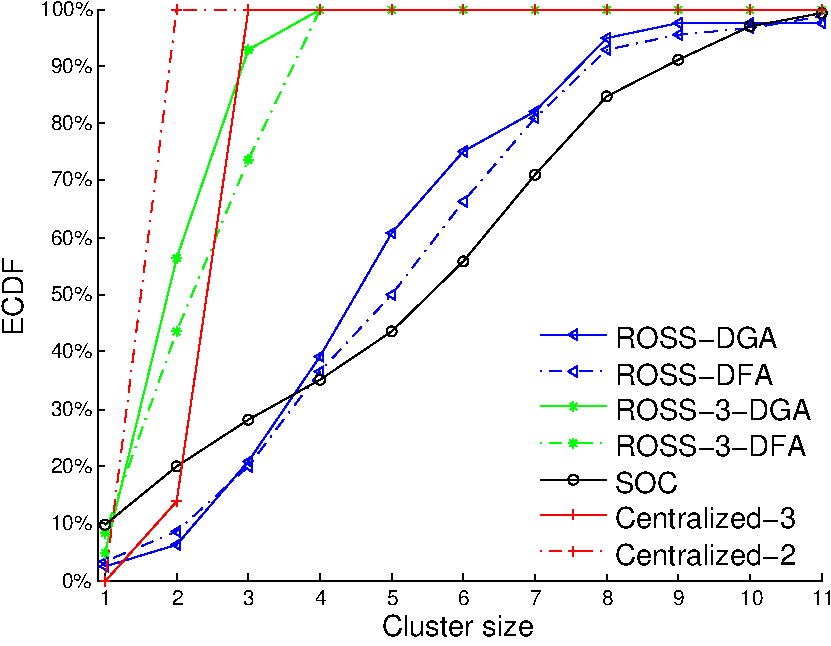
\includegraphics[width=0.8\linewidth]{cdf_clusterSize_20.pdf}
  \caption{Distribution of CRs residing in clusters with different sizes, as to ROSS with size control feature, the desired cluster size is 3. The average number of neighbours is 4.838.}
  \label{size_control}
\end{figure}
Figure~\ref{size_control} shows the number of CRs residing in certain sized clusters.
The centralized schemes are able to form clusters which strictly satisfy the requirement on cluster sizes.
When the desired size is 2, each generated cluster has two members.
When the desired size is 3, in average only 3 CRs are formed into 2 node clusters.
When ROSS-3-DFA is applied, most number of CRs are in 3 node clusters, nevertheless, slightly less nodes are found in 2 node and 4 node clusters, there are also considerable number of singleton clusters.
ROSS-3-DGA decreases the clusters sizes and results in more 2 node clusters, the second most CRs are found in 3 node clusters.
ROSS-DGA and ROSS-DFA generate rather even distribution of nodes with different sizes, whereas SOC results in more CRs unclustered or clusters of large sizes. 
Figure~\ref{size_control} shows distributed clustering schemes are not able to control cluster sizes perfectly, but ROSS-DGA and ROSS-DFA eliminate the clusters whose size diverges largely with the desired one, \ie single node clusters and clusters with size of 13 and 14.
Particularly, size control enable both ROSS-DGA and ROSS-DFA to achieve clusters whose sizes demonstrate certain homogeneity, \ie cluster sizes vary from 1 to 4.
But there are considerable number of single node clusters, which is due to the cluster pruning discussed in section~\ref{cluster_pruning}.

\subsubsection*{Control Signalling Overhead}
%Different from the clustering schemes proposed in ~\cite{LIU_TMC11_2, clustering_globecom11}, 
As to any variants of ROSS, there are two phases, in the first phase, clusters are formed, in the second phase, cluster membership is decided so that each node only resides in one cluster.
Control message exchanges between CR nodes are involved in both phases.

In this section we compare the amount of control messages involved for clustering in different schemes, \eg centralized scheme, ROC, ROSS-DGA, ROSS-DFA and those with size control feature.
In order to highlight the amount of control signalling only for clustering, we omit the control messages used for neighbourhood discovery, which are regarded the same for all schemes, and only compare the number of control messages brought in by the features of the schemes. 
The control message here refers both broadcast and unicast.

As to variants of ROSS, in the first phase, after each node broadcasts their new knowledge on spectrum robustness, cluster is automatically formed by cluster head which is decided from consensus by comparing the spectrum robustness with neighbours, then the cluster head broadcasts message containing its ID and the available channels in its cluster.
As to ROSS with size control feature, there are same amount of cluster heads with ROSS without enabling size control feature, and the cluster head broadcasts the available channels of the pruned cluster.
Afterwards in the second phase, membership clarification of debatable nodes is conducted.
Debatable node informs the cluster which it going to stay and the cluster head broadcasts message about its new cluster.
As to SOC, each node needs to maintain one cluster, the final clusters are formed after three rounds of comparisons and cluster mergers, while as to ROSS, only debatable nodes need to communicate with cluster heads to clarify their membership.
%1. update membership to form X1, 
%2. broadcast new X1, form new X2
%3. broadcast X3

Worst case protocol complexities.
We assume that the protocols execute synchronously. 
We compare the Time Complexity (\gls{TC}), defined as the number of steps required to perform a protocol operation, and the Communication Complexity (CC), defined as the number of broadcast in performing the operation.

The complexity parameters are the number of nodes $n$ in network, number of clusters $h$.

The quantitative analysis of amount of control overhead and the size of messages are illustrated in Table \ref{tab_overhead}, 

\begin{table}[hc]
\center
\begin{tabular}{|p{3 cm}|p{3 cm}|p{7.5 cm}|}
\hline
 Scheme 		&   Number of broadcast  	& Content of message \\ \hline
 ROSS-DGA, ROSS-x-DGA 		&   $h+2*m^2c$  (upper bound)				& $ID_{H_C}$ and $V_C$ for $h+m^2c$ times, notification to join in one cluster for $m^2c$ times					\\ \hline
 ROSS-DFA, ROSS-x-DFA 		&   $h+ 2m$	 (upper bound)				& $ID_{H_C}$ and $V_C$ for $h+m$ times, notification to join in one cluster for $m$ times	 					\\ \hline
 SOC 			&   $3*n$					& $\{V_i\}, i\in M\subseteq Nb_i$						\\ \hline
 Centralized	&	$n$						& $\{C\}$         	\\ \hline
\end{tabular}
\caption{Singalling overhead. Notations: $n$-number of CR nodes in CRN, $h$-number of cluster heads, $m$-number of debatable nodes, $c$-number of demanding clusters, $\delta$-desired cluster size}
\label{tab_overhead}
\end{table}


\begin{figure}[ht!]
  \centering
  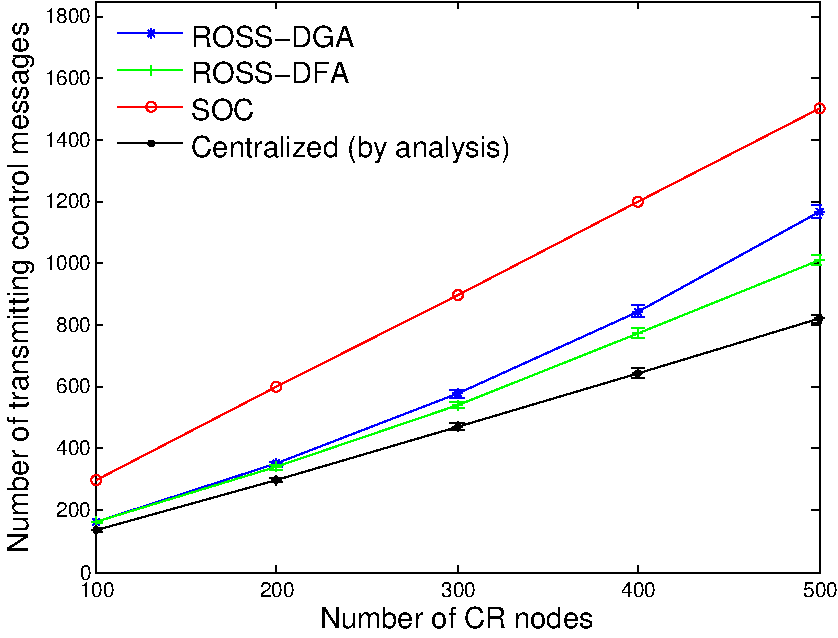
\includegraphics[width=0.67\linewidth]{number_controlMsg.pdf}
  \caption{Number of control messages}
  \label{control_msg}
\end{figure}


\subsection{Comparison between Distributed Schemes}
In this part we investigate the performances of distributed schemes in CRN with different network scales and densities.
The transmission range for CR is $A/10$ whereas $A/5$ for PR.
The number of PU is 30, we investigate the CRN where number of CR is 100, 200 and 300, and the average number of neighbours of each CR is 9.5, 20, and 31.


\subsubsection*{Number of CCC per Non-singleton Clusters}

\begin{figure}[ht!]
  \centering
  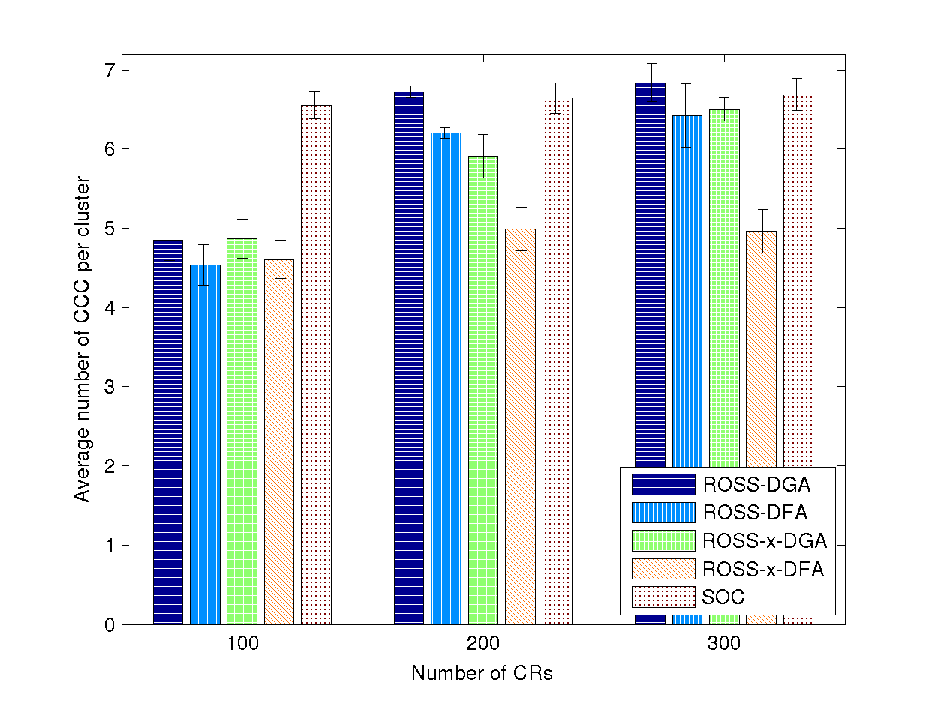
\includegraphics[width=1\linewidth]{ccc_large_scale_color.pdf}
  \caption{Number of common channels for non-singleton clusters. As to ROSS with size control feature, we adopt $x=6$ when $N=100$, $x=12$ when $N=200$, $x=21$ when $N=300$, which is around $2/3$ of the number of average neighbours}
  \label{ccc_large_scale}
\end{figure}

Figure~\ref{ccc_large_scale} illustrates the average number of CCCs of the non-singleton clusters.
It shows when $N=100$, variants of ROSS have 30\% less CCCs than SOC, but this gap is decreased significantly when $N$ is 200 and 300, \ie when $N=300$, number of CCCs achieved by ROSS variants (except for ROSS-x-DFA) is almost the same with that resulted from SOC.

This means SOC performs better on average number of CCCs per non-singleton clusters when network density is small~\footnote{this is also observed in the evaluation in Section \ref{ccc_20} where $N=20$}, when the network becomes denser, ROSS-DGA achieves even more CCCs than SOC, and ROSS-DFA and ROSS-x-DGA visibly increase their performances on the number of CCCs.




\subsubsection*{Survival Rate of Clusters with Increasing Primary Users}
With the increase of PRs in the network, some clusters will lose certain CCCs as these CCCs are no longer available on certain cluster members.
When there is no CCCs available in a cluster, the cluster is said to be broken.
In this part of simulation, we investigate the robustness of clusters by increasing the PRs working on certain channels.
 
Figure~\ref{singleton_clusters_100} shows the increasing tread of singleton clusters, or to say, unclustered nodes, with the increase of PRs.
SOC generates around 10 more singleton clusters than the variants of ROSS, which accounts for 10\% of the total CR nodes.
The confidence intervals of the variants of ROSS are not shown in the figure as they overlap, and we only show the average values.
It can be seen that greedy algorithms result in slightly less singleton clusters than their counterparts.

Figure ~\ref{singleton_clusters_300} shows a more dense CRN where $N=300$.
SOC noticeably causes more singleton clusters than ROSS variants, except that ROSS-3-DFA results in more singleton clusters when PRs are few.
The reason is that ROSS-3-DFA conducts cluster membership clarification for only once, which causes large number of singleton clusters, while, in ROSS-3-DGA increase the size of smaller clusters through debatable nodes' repeated updates thus drastically decreases the number of singleton clusters.

\begin{figure}[h!]
  \centering
  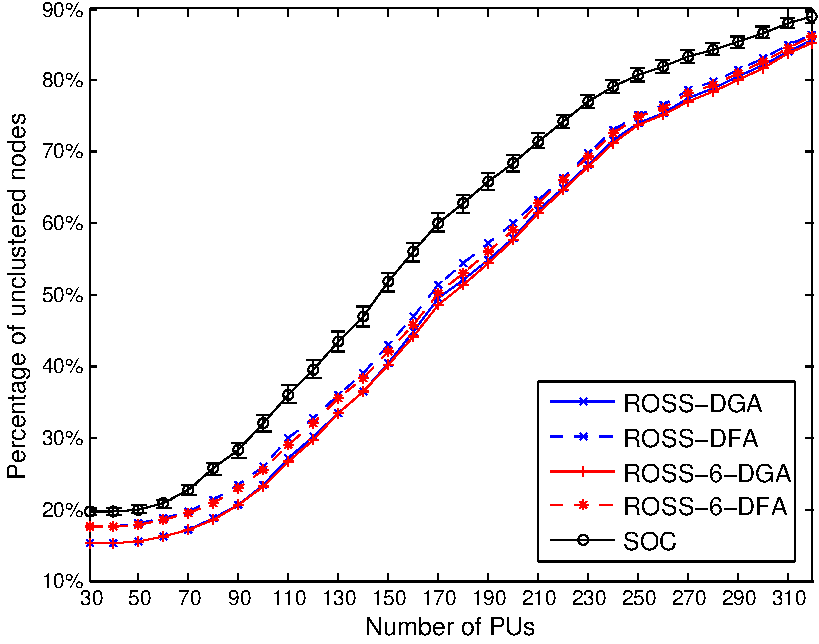
\includegraphics[width=0.8\linewidth]{survival_rate_100.pdf}
  \caption{Number of CRs which are not included in any clusters, $N=100$}
  \label{singleton_clusters_100}
   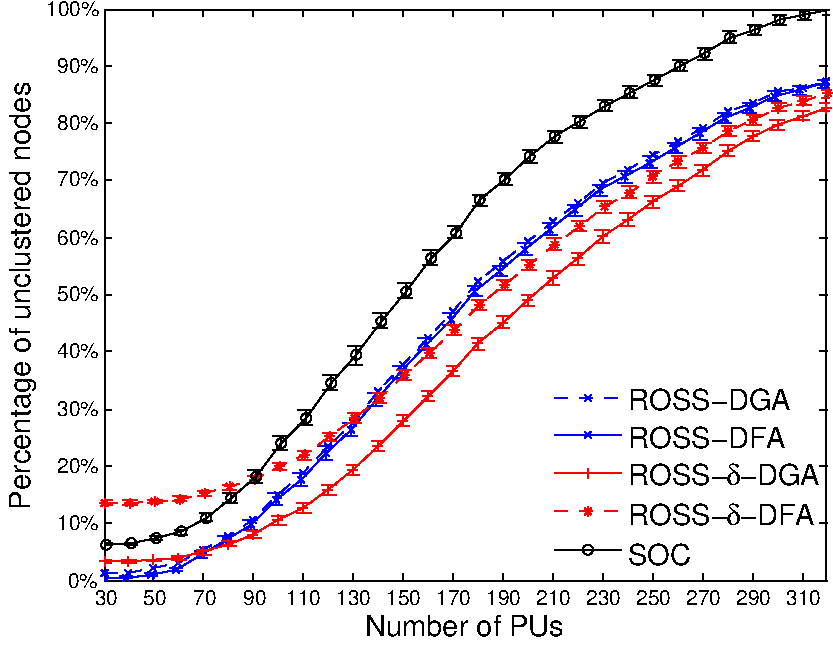
\includegraphics[width=0.8\linewidth]{survival_rate_300.pdf}
  \caption{Number of CRs which are not included in any clusters, $N=300$}
  \label{singleton_clusters_300}
\end{figure}

From the Figure~\ref{singleton_clusters_100} and \ref{singleton_clusters_300}, we can conclude that the greedy versions of ROSS are more robust than their counterpart variants of ROSS.
When the network is more dense, the improvement on cluster sizes and robustness by the greedy search in the membership clarification phase is more obvious.


\subsubsection*{Cluster Size Control}

The number of formed clusters is shown in Fig.~\ref{nClusters_largeNetwork}.
When the network scales up, the number of formed clusters by ROSS increases by smaller margin.
This result coincides with the analysis in Section~\ref{cluster_pruning}, that with ROSS, the number of formed clusters saturates when the network scales.
When the network becomes denser, more clusters are generated by SOC compared with ROSS variants.
To better understand the distribution of the sizes of formed clusters, we depict the cluster sizes with cumulative distribution.
In this group of evaluation, the number of PRs is 30.

\begin{figure}[h]
  \centering
   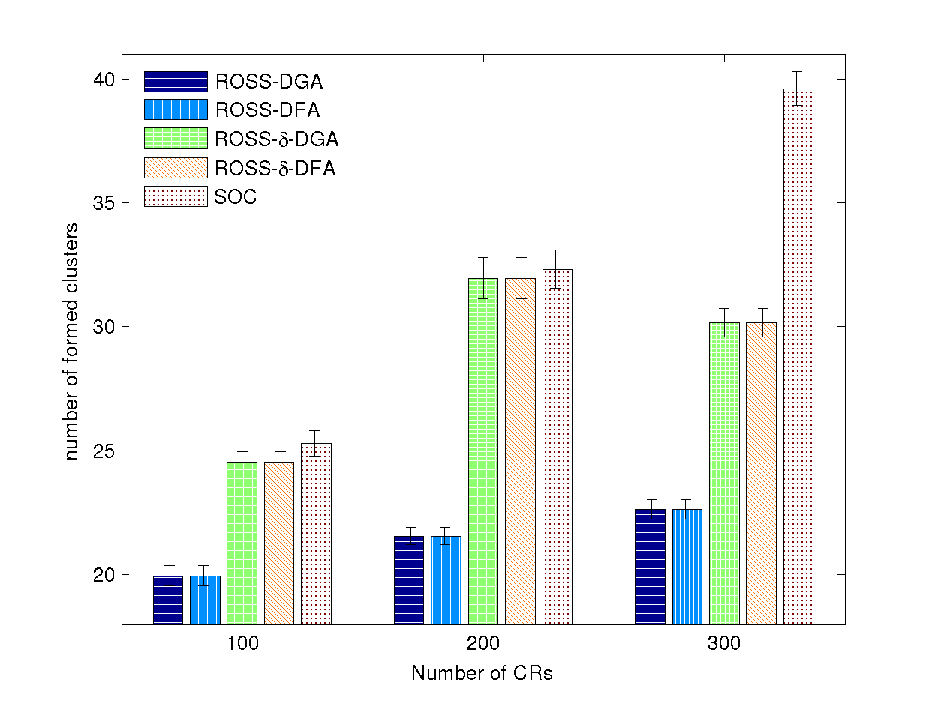
\includegraphics[width=0.85\linewidth]{nClusters_largeNetwork.pdf}
  \caption{Number of formed clusters}
  \label{nClusters_largeNetwork}
\end{figure}





%\begin{figure}[ht]
%\begin{center}
%%\centering
%\subfigure[100 CRs, 30 PRs]{\label{result1:1}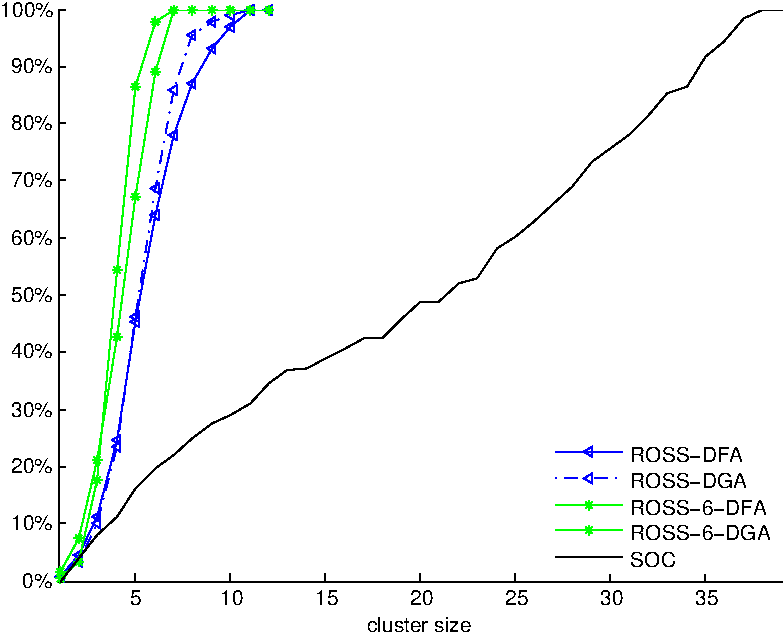
\includegraphics[width=0.48\linewidth]{cdf_clusterSize_100.pdf}}
%\subfigure[300 CRns, 30 PRns]{\label{result1:2}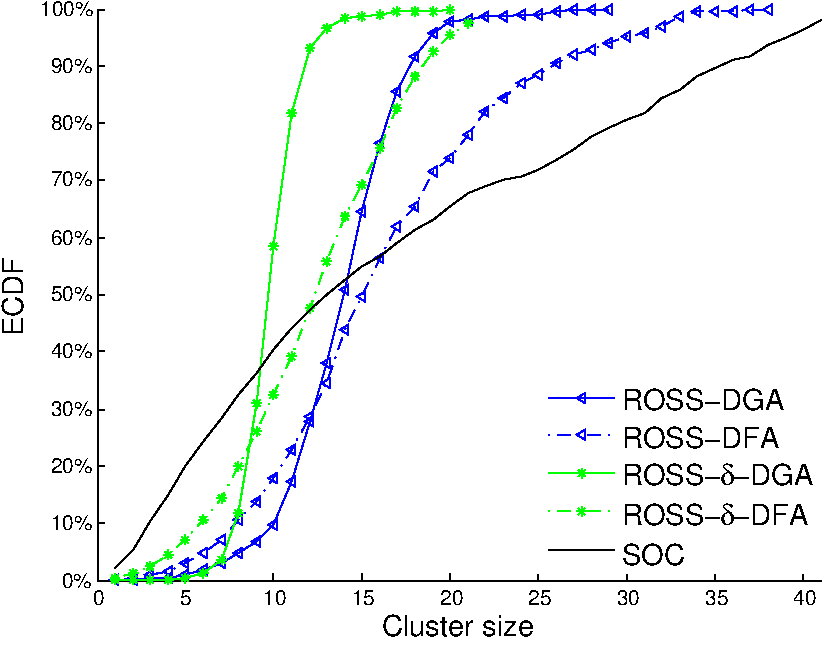
\includegraphics[width=0.48\linewidth]{cdf_clusterSize_300.pdf}}
%\end{center} 
%\caption[Cluster sizes]{Distribution of CRs in clusters with different sizes} %{\subref{a}, \subref{b}, \subref{c}, \subref{d}}
%\label{result1}
%\end{figure}

Figure~\ref{cdf_clusterSize_100} illustrates the distribution of CR nodes which reside in clusters with certain sizes.
When variants of ROSS are applied, most CRs are included into clusters with sizes between 2 and 5, in particular, ROSS-2-DGA achieves homogeneous distribution of cluster sizes, \ie, there is no cluster whose size is greater than 3, and the number of CRs in 2 node cluster is greater than that resulted from ROSS-2-DFA.
xxxxxxxxxxxxxxxxxxxxxxxxxxxxxxxxxxx(modify the plots, and the words)xxxxxxxxxxx
This is because in membership clarification phase, greedy search not only increases the number of CCCs of relevant clusters, but is liable to leave debatable nodes to stay in smaller clusters, as stated in Algorithm~\ref{alg4}.
SOC doesn't have size control feature, thus the cluster sizes diverge strongly, \ie the sizes span from 1 to 35.

\begin{figure}[h]
  \centering
   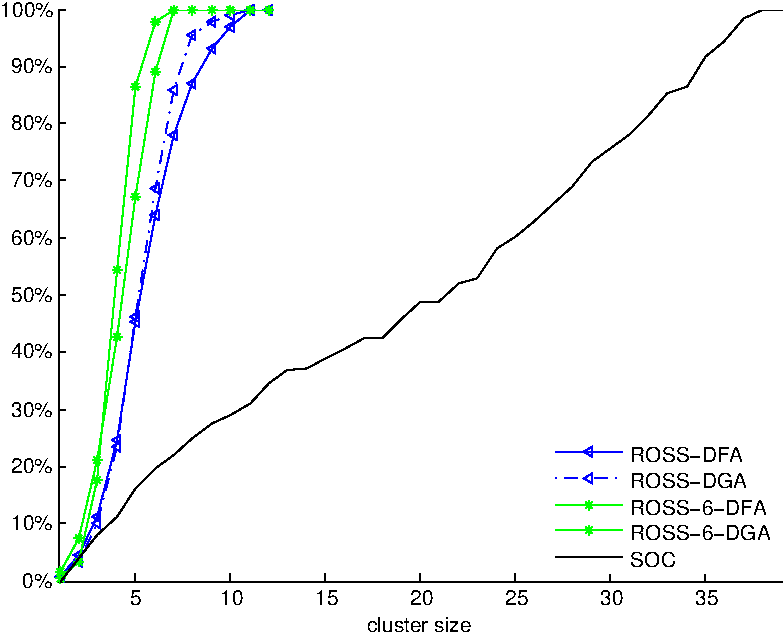
\includegraphics[width=0.7\linewidth]{cdf_clusterSize_100.pdf}
  \caption{100 CRs, 30 PRs, the average number of neighbours is 9.5.}
  \label{cdf_clusterSize_100}
\end{figure}

\begin{figure}[h]
  \centering
   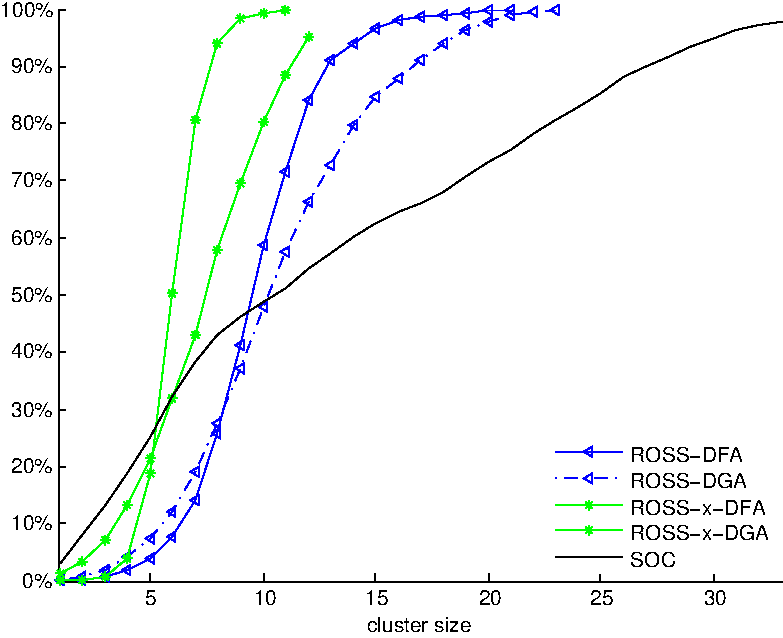
\includegraphics[width=0.7\linewidth]{cdf_clusterSize_200.pdf}
  \caption{200 CRs, 30 PRs, the average number of neighbours is 20}
  \label{cdf_clusterSize_200}
\end{figure}




In a denser network with 300 CRs as shown in Figure~\ref{cdf_clusterSize_300}, where desired size is 3, 94\% of CRs are integrated into 2 or 3 node clusters by ROSS-3-DGA, as to ROSS-3-DFA, 13\% CRs constitute singleton clusters, and 27\% CRs are within 4 node clusters.
Cluster size spans over a large range for schemes which don't have cluster size control mechanism.
As to ROSS-DGA, ROSS-DFA and SOC, 95\% of CRs stay in clusters whose sizes are smaller than 8, 9 and 14 respectively.

\begin{figure}[h]
  \centering
   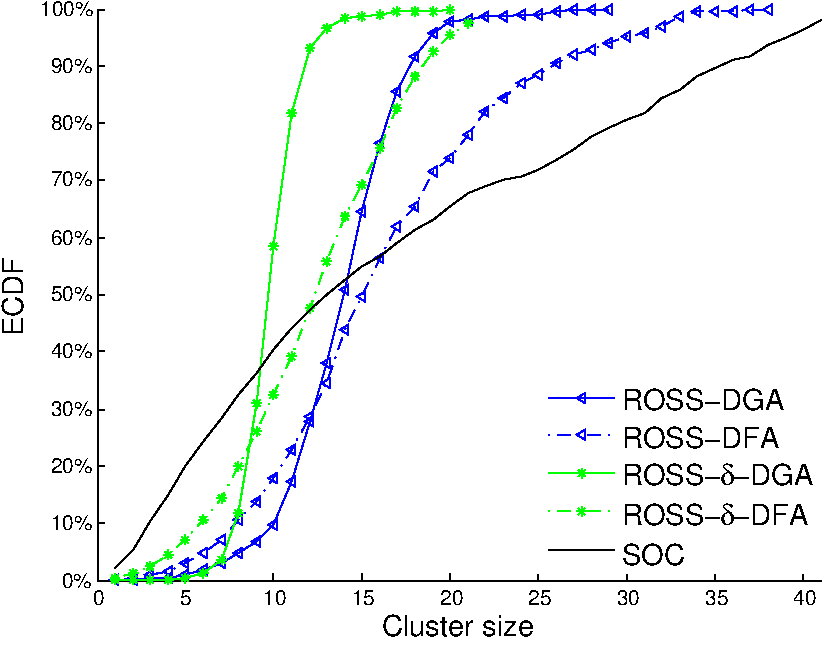
\includegraphics[width=0.7\linewidth]{cdf_clusterSize_300.pdf}
  \caption{300 CRs, 30 PRs, the average number of neighbours is 30}
  \label{cdf_clusterSize_300}
\end{figure}


\begin{comment}
In the first case, there are 100 CR nodes while primary users are increased from 10 to 150. More primary users lead to fewer idle channels available in the whole network, and thus cause a challenge to the formation of clusters. In Figure~\ref{result1:1}, the average number of inner common channels achieved by the three approaches decreases with increasing the number of primary users. ROSS-DGA/DFA outperform SOC by at most $15\%$ in this case.
In Figure~\ref{result1:2}, we present the average number of outward common channels. Here, ROSS-DFA outperforms SOC by $20\%$-$40\%$ due to putting CR nodes with bigger connectivity degree at the border of clusters to strengthen the connection among them. % while the advantage of ROSS increases the more primary users are active. 
ROSS-DGA performs slightly better than ROSS-DFA on the whole range due to its larger number of iterations.

For the second scenario, we vary the number of CR nodes from 100 to 500 while keeping the number of primary users fixed at 100. Hence, we investigate the behavior of the three schemes in sparse and dense situations. Figure~\ref{result2:1} shows the average number of ICCs. We observe that ROSS-DGA/DFA achieves more CCCs in sparse networks while slightly less in dense networks. We attribute this to two reasons, firstly, SOC pursues the maximal product of cluster size and number of ICC, so the product value is assured in many cases by decreasing cluster size to get more ICCs. Actually, there is a large number of clusters with only one member. %Figure \ref{result3:2} shows that the number of such clusters delivered by SOC is 120\% more than that of ROSS. 
Secondly, ROSS-DGA/DFA builds clusters on the basis of one-hop neighborhood, and dense network means there are more CR nodes within the neighborhood, thus agree on less ICCs. Figure~\ref{result2:2} demonstrates an increasing advantage of ROSS-DGA/DFA against SOC on number of outward common channels, because more nodes with bigger connectivity degree are put as border nodes. The distribution of cluster sizes are presented in Figure~\ref{result3:1} and \ref{result3:2} with variation of density. We observe that clusters formed by ROSS-DGA/DFA have similar size. Note in particular that the number of one-node clusters generated by SOC is much bigger than that produced by ROSS-DGA/DFA in both cases. This becomes especially a problem as the density increases. 

Compared with ROSS-DGA, we can find from the simulation that ROSS-DFA has much less complexity by scarifying a little performance, and both ROSS-DGA and ROSS-DFA are less complex that SOC which has a complexity of the order of $\vert I\vert^4$. This was confirmed by the run times of the simulations, which were significantly longer when simulating SOC.

\begin{figure}[t]
\begin{center}

%\centering
\subfigure[100 PRns, varying CRns]{\label{result2:1}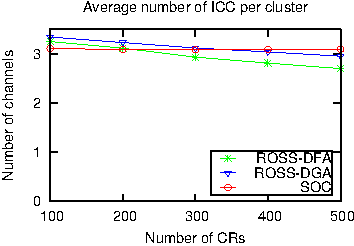
\includegraphics[width=0.45\linewidth]{CR_ICC_3curves.pdf}}
\subfigure[100 PRns, varying CRns]{\label{result2:2}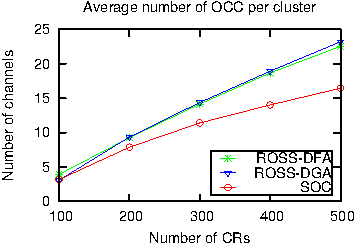
\includegraphics[width=0.45\linewidth]{CR_OCC_3curves.pdf}}
 \end{center}
\caption[]{Connectivity robustness of ICCs and OCCs with varying density of CR nodes.} %\subref{node A in $C_C$}, \subref{node A in $C_H$}}
\label{result2}
\end{figure}

\begin{figure}[ht!]
\begin{center}
%\centering
\subfigure[100 CRns, 100 PRns]{\label{result3:1}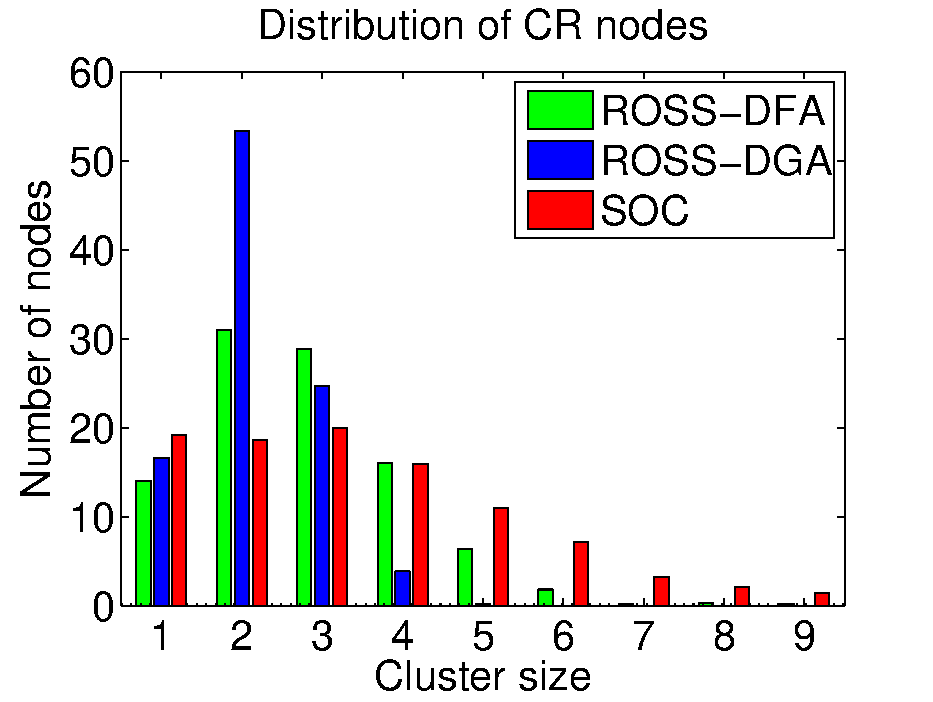
\includegraphics[width=0.45\linewidth]{distribution_1_matlab.pdf}}
\subfigure[200 CRns, 100 PRns]{\label{result3:2}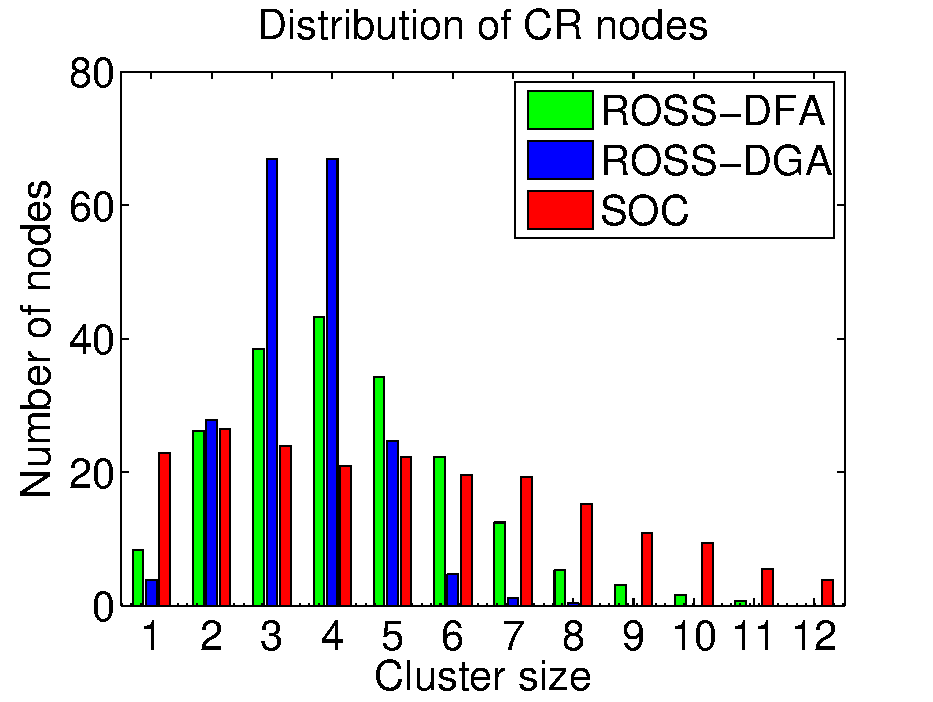
\includegraphics[width=0.45\linewidth]{distribution_2_matlab.pdf}}
 \end{center}
\caption[]{Distribution of cluster sizes for two fixed scenarios.} %\subref{node A in $C_C$}, \subref{node A in $C_H$}}
\label{result3}
\end{figure}	

\end{comment}


\section{Conclusions and Future Work}
\label{conclusion}
We investigate extensively the robust clustering problem in CRN, which is important to form clusters which maintains unbroken to the greatest extent possible under primary users' activity.
We prove the NP hardness of the problem and one distributed and light weighted clustering scheme ROSS-DGA is proposed.
The clusters resulted from ROSS-DGA and its faster version ROSS-DFA are less vulnerable compared with other distributed clustering schemes, and demonstrates similar survival rate with centralized scheme under primary users' influence.
An light weighted cluster size control mechanism is contained in both ROSS-DGA and ROSS-DFA, which is advantageous for cooperative sensing and network operation with clusters.
Furthermore, considerable less control messages are generated when compared with other clustering schemes.

The drawback of this scheme is it does not form big clusters, which is attributed to that ROSS forms cluster based on cluster head's neighbourhood, and does not absorb CR nodes outside of the neighbourhood.
Big clusters could be demanded when the network density is low.

%Our work is in process, in which a light weighted clustering scheme is proposed. Intra connectivity is ensured by the border nodes, which has larger number of common channels with its neighbors within its vicinity, inter connectivity is guaranteed by deleting certain one-hop away nodes out of clusters to increase the set of common channels by a game theory approach. In this way, bigger value of  $\bar{N_{inter}}\times\bar{N_{intra}}$ could be achieved. 

%There are several issues can be investigated on the basis of current work of spectrum sharing. Firstly, as our scheme adapts multi-radio communication, channel assignment within and between clusters can be implemented to decrease interferences caused by co-channel interferences, this topic is pretty new in the scenario of cognitive radio. Secondly, the second phase of our clustering scheme can be optimized by letting nodes locating in more than one cluster use coalitional strategies, although the complexity could be higher. Thirdly, the number of the neighboring nodes is not considered when deciding cluster heads, which need to be examined in the future.
